\section{Area Between Curves}\label{sec:AreaBetweenCurves}



We begin this chapter with a reminder of a few key concepts discussed thus far. Let $f$ be a continuous function on $[a,b]$ which is partitioned into $n$ equally spaced subintervals as $$a<x_1 < x_2 < \cdots < x_n<x_{n+1}=b.$$ Let $\dx=(b-a)/n$ denote the length of the  subintervals, and let $c_i$ be any $x$-value in the $i^\text{ th}$ subinterval. Definition \ref{def:rie_sum} states that the sum $$\sum_{i=1}^n f(c_i)\dx$$ is a \textit{Riemann Sum.} Riemann Sums are often used to approximate some quantity (area, volume, work, pressure, etc.). The \textit{approximation} becomes \textit{exact} by taking the limit 
$$\lim_{n\to\infty} \sum_{i=1}^n f(c_i)\dx.$$ Theorem \ref{thm:riemann_sum} connects limits of Riemann Sums to definite integrals:
$$\lim_{n\to\infty} \sum_{i=1}^n f(c_i)\dx = \int_a^b f(x)\ dx.$$ Finally, the Fundamental Theorem of Calculus states how definite integrals can be evaluated using antiderivatives. 

This chapter employs the following technique to a variety of applications. Suppose the value $Q$ of a quantity is to be calculated. We first approximate the value of $Q$ using a Riemann Sum, then find the exact value via a definite integral. We spell out this technique in the following Key Idea.


\begin{formulabox}[\label{idea:app_of_defint} Application of Definite Integrals Strategy ]
{Let a quantity be given whose value $Q$ is to be computed.\index{integration!general application technique}
\begin{enumerate}
\item		Divide the quantity into $n$ smaller ``subquantities'' of value $Q_i$.
\item		Identify a variable $x$ and function $f(x)$ such that each subquantity can be approximated with the product $f(c_i)\dx$, where $\dx$ represents a small change in $x$. Thus $Q_i \approx f(c_i)\dx$. A sample approximation $f(c_i)\dx$ of $Q_i$ is called a \textit{differential element}.
\item		Recognize that $\ds Q= \sum_{i=1}^n Q_i \approx \sum_{i=1}^n f(c_i)\dx$, which is a Riemann Sum.
\item		Taking the appropriate limit gives $\ds Q = \int_a^b f(x)\ dx$
\end{enumerate}
}
\end{formulabox}


This Key Idea will make more sense after we have had a chance to use it several times. We begin with Area Between Curves.
%\end{minipage}
\clearpage

\section*{Area Between Curves}\label{sec:ABC}

We are often interested in knowing the area of a region. Forget momentarily that we discussed this already in Section  \ref{chapter:integration}.\ref{sec:FTC} and approach it instead using the technique described in Key Idea \ref{idea:app_of_defint}. 

Let $Q$ be the area of a region bounded by continuous functions $f$ and $g$. If we break the region into many subregions, we have an obvious equation:

\hfill Total Area = sum of the areas of the subregions. \hfill \null

The issue to address next is how to systematically break a region into subregions. A graph will help. Consider Figure \ref{fig:abcintro} (a) where a region between two curves is shaded. While there are many ways to break this into subregions, one particularly efficient way is to ``slice'' it vertically, as shown in Figure \ref{fig:abcintro} (b), into $n$ equally spaced slices. 

We now approximate the area of a slice. Again, we have many options, but using a rectangle seems simplest. Picking any $x$-value $c_i$ in the $i^\text{ th}$ slice, we set the height of the rectangle to be $f(c_i)-g(c_i)$, the difference of the corresponding $y$-values. The width of the rectangle is a small difference in $x$-values, which we represent with $\dx$. Figure \ref{fig:abcintro} (c) shows sample points $c_i$ chosen in each subinterval and appropriate rectangles drawn. (Each of these rectangles represents a differential element.) Each slice has an area approximately equal to $\big(f(c_i)-g(c_i)\big)\dx$; hence, the total area is approximately the Riemann Sum
$$Q = \sum_{i=1}^n \big(f(c_i)-g(c_i)\big)\dx.$$
Taking the limit as $n\to \infty$ gives the exact area as $\int_a^b \big(f(x)-g(x)\big)\ dx.$


\begin{figure}
	\centering
	\begin{subfigure}{0.33\textwidth}
		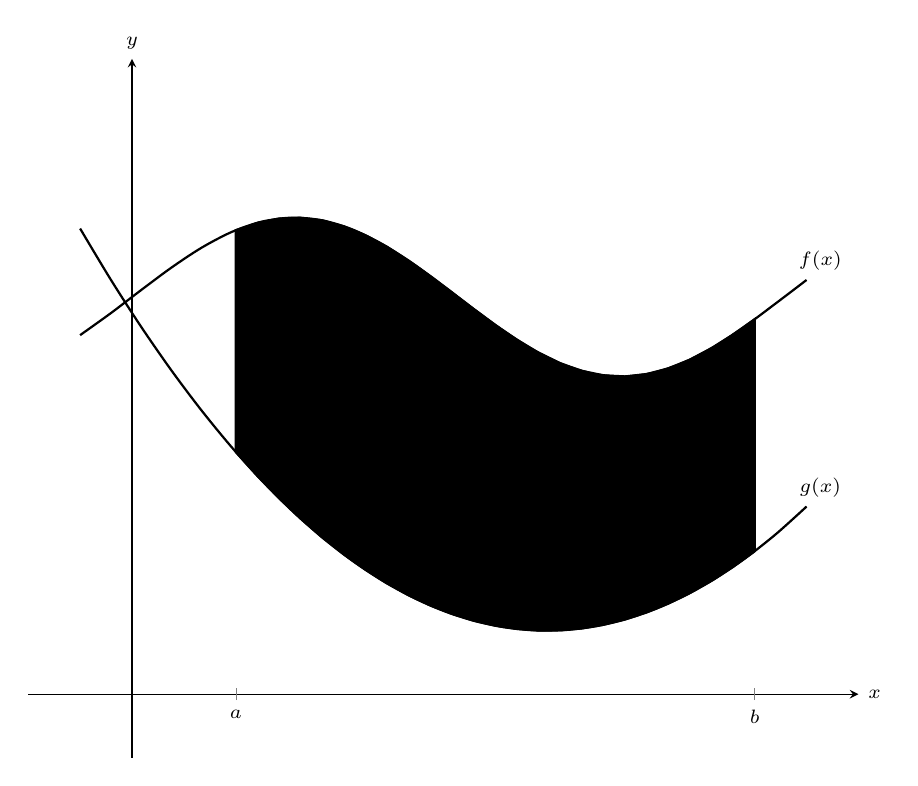
\begin{tikzpicture}
		\begin{axis}[width=\textwidth,%
		tick label style={font=\scriptsize},axis y line=middle,axis x line=middle,name=myplot,axis on top,%
					%x=.37\marginparwidth,
					%y=.37\marginparwidth,
					xtick=\empty,% 
					extra x ticks={.5,3},
					extra x tick labels={$a$,$b$},
					ytick=\empty,
					%minor y tick num=1,%extra y ticks={-5,-3,...,7},%
		%			minor x tick num=4,
					ymin=-.2,ymax=2,%
					xmin=-.5,xmax=3.5%
		]
		
		\addplot [{\coloronefill},domain=.5:3,stack plots=y] {.25*(x-2)^2+.2};
		\addplot [{\coloronefill},thick,fill={\coloronefill},area style,domain=.5:3,stack plots=y] {.25*sin(deg(2*x))+1.25-(.25*(x-2)^2+.2)} \closedcycle;
		\addplot [smooth,thick, {\colorone},domain=-.25:3.25] {.25*sin(deg(2*x))+1.25} node [shift={(5pt,7pt)} ,black] {\scriptsize $f(x)$};
		\addplot [smooth,thick, {\colorone},domain=-.25:3.25] {.25*(x-2)^2+.2}node [shift={(5pt,7pt)} ,black] {\scriptsize $g(x)$};
		
		
		\end{axis}
		
		\node [right] at (myplot.right of origin) {\scriptsize $x$};
		\node [above] at (myplot.above origin) {\scriptsize $y$};
		\end{tikzpicture}
        \label{fig:figabcintroa}
        \caption{} 
    \end{subfigure}% 
    \begin{subfigure}{0.33\textwidth}
    \include{figures/figabcintrob.tex}
        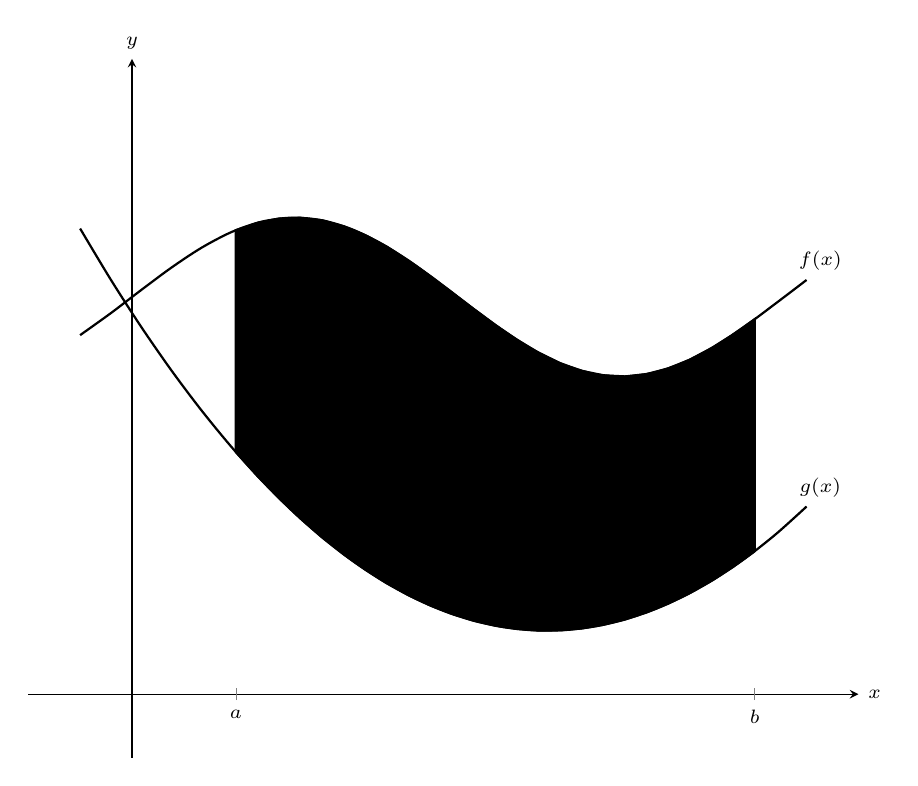
\begin{tikzpicture}
        \begin{axis}[width=\textwidth,%
        tick label style={font=\scriptsize},axis y line=middle,axis x line=middle,name=myplot,axis on top,%
        			%x=.37\marginparwidth,
        			%y=.37\marginparwidth,
        			xtick=\empty,% 
        			extra x ticks={.5,3},
        			extra x tick labels={$a$,$b$},
        			ytick=\empty,
        			%minor y tick num=1,%extra y ticks={-5,-3,...,7},%
        %			minor x tick num=4,
        			ymin=-.2,ymax=2,%
        			xmin=-.5,xmax=3.5%
        ]
        
        \addplot [{\coloronefill},domain=.5:3,stack plots=y] {.25*(x-2)^2+.2};
        \addplot [{\coloronefill},thick,fill={\coloronefill},area style,domain=.5:3,stack plots=y] {.25*sin(deg(2*x))+1.25-(.25*(x-2)^2+.2)} \closedcycle;
        \addplot [smooth,thick, {\colorone},domain=-.25:3.25] {.25*sin(deg(2*x))+1.25} node [shift={(5pt,7pt)} ,black] {\scriptsize $f(x)$};
        \addplot [smooth,thick, {\colorone},domain=-.25:3.25] {.25*(x-2)^2+.2}node [shift={(5pt,7pt)} ,black] {\scriptsize $g(x)$};
        
        \draw [thick] (axis cs:0.5,0.7625)--(axis cs:0.5,1.46) (axis cs:1.,0.45)--(axis cs:1.,1.477) (axis cs:1.5,0.2625)--(axis cs:1.5,1.285) (axis cs:2.,0.2)--(axis cs:2.,1.061) (axis cs:2.5,0.2625)--(axis cs:2.5,1.01) (axis cs:3.,1.18)--(axis cs:3.,0.45) (axis cs:0.75,1.499)--(axis cs:0.75,0.5906) (axis cs:1.25,0.3406)--(axis cs:1.25,1.4) (axis cs:1.75,1.162)--(axis cs:1.75,0.2156) (axis cs:2.25,0.2156)--(axis cs:2.25,1.006) (axis cs:2.75,1.074)--(axis cs:2.75,0.3406);
        
        %(0.5,0.7625)(1.,0.45)(1.5,0.2625)(2.,0.2)(2.5,0.2625)(3.,0.45)
        %(0.5,1.46)(1.,1.477)(1.5,1.285)(2.,1.061)(2.5,1.01)(3.,1.18)
        
        %(0.75,0.5906)(1.25,0.3406)(1.75,0.2156)(2.25,0.2156)(2.75,0.3406)
        %(0.75,1.499)(1.25,1.4)(1.75,1.162)(2.25,1.006)(2.75,1.074)
        \end{axis}
        
        \node [right] at (myplot.right of origin) {\scriptsize $x$};
        \node [above] at (myplot.above origin) {\scriptsize $y$};
        \end{tikzpicture}
        \caption{}    
    \end{subfigure} 
    
    \begin{subfigure}{0.33\textwidth}
        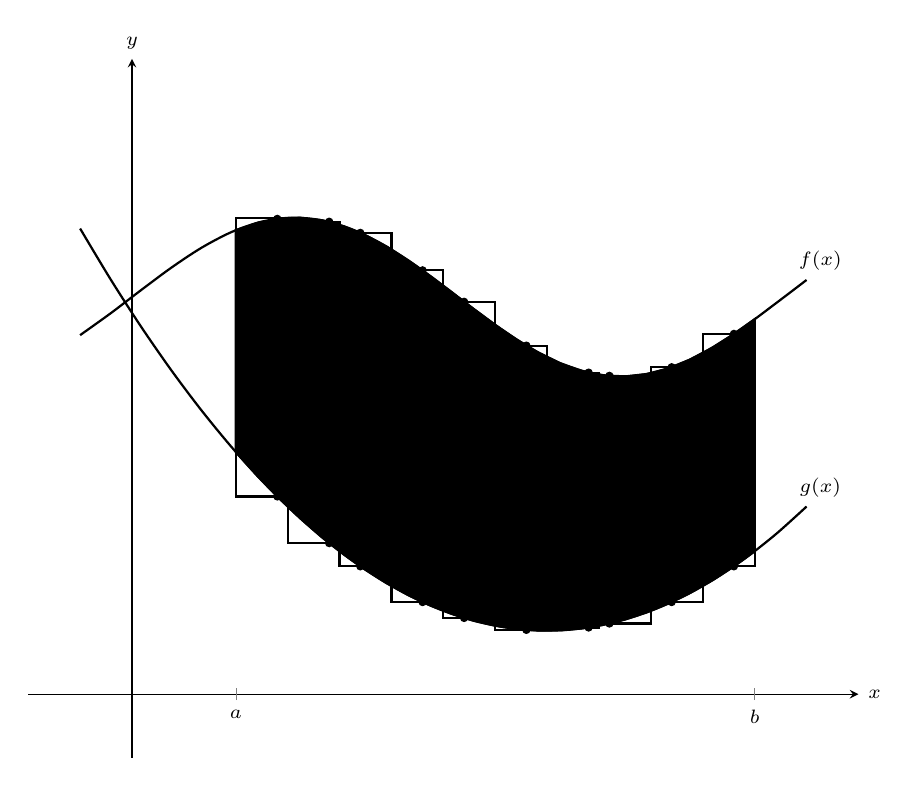
\begin{tikzpicture}
        \begin{axis}[width=\textwidth,%
        tick label style={font=\scriptsize},axis y line=middle,axis x line=middle,name=myplot,axis on top,%
        			%x=.37\marginparwidth,
        			%y=.37\marginparwidth,
        			xtick=\empty,% 
        			extra x ticks={.5,3},
        			extra x tick labels={$a$,$b$},
        			ytick=\empty,
        			%minor y tick num=1,%extra y ticks={-5,-3,...,7},%
        %			minor x tick num=4,
        			ymin=-.2,ymax=2,%
        			xmin=-.5,xmax=3.5%
        ]
        
        \addplot [{\coloronefill},domain=.5:3,stack plots=y] {.25*(x-2)^2+.2};
        \addplot [{\coloronefill},thick,fill={\coloronefill},area style,domain=.5:3,stack plots=y] {.25*sin(deg(2*x))+1.25-(.25*(x-2)^2+.2)} \closedcycle;
        \addplot [smooth,thick, {\colorone},domain=-.25:3.25] {.25*sin(deg(2*x))+1.25} node [shift={(5pt,7pt)} ,black] {\scriptsize $f(x)$};
        \addplot [smooth,thick, {\colorone},domain=-.25:3.25] {.25*(x-2)^2+.2}node [shift={(5pt,7pt)} ,black] {\scriptsize $g(x)$};
        
        %\draw [thick] (axis cs:0.5,0.7625)--(axis cs:0.5,1.46) (axis cs:1.,0.45)--(axis cs:1.,1.477) (axis cs:1.5,0.2625)--(axis cs:1.5,1.285) (axis cs:2.,0.2)--(axis cs:2.,1.061) (axis cs:2.5,0.2625)--(axis cs:2.5,1.01) (axis cs:3.,1.18)--(axis cs:3.,0.45) (axis cs:0.75,1.499)--(axis cs:0.75,0.5906) (axis cs:1.25,0.3406)--(axis cs:1.25,1.4) (axis cs:1.75,1.162)--(axis cs:1.75,0.2156) (axis cs:2.25,0.2156)--(axis cs:2.25,1.006) (axis cs:2.75,1.074)--(axis cs:2.75,0.3406);
        
        \draw [thick] (axis cs:0.5,0.6225)rectangle(axis cs:0.75,1.5) (axis cs:1.,1.487)rectangle(axis cs:0.75,0.4756) (axis cs:1.,0.4025)rectangle(axis cs:1.25,1.452) (axis cs:1.5,1.334)rectangle(axis cs:1.25,0.29) (axis cs:1.5,0.24)rectangle(axis cs:1.75,1.235) (axis cs:2.,1.097)rectangle(axis cs:1.75,0.2025) (axis cs:2.,0.21)rectangle(axis cs:2.25,1.012) (axis cs:2.5,1.002)rectangle(axis cs:2.25,0.2225) (axis cs:2.5,0.29)rectangle(axis cs:2.75,1.029)(axis cs:3.,1.134)rectangle(axis cs:2.75,0.4025);
        
        \filldraw (axis cs:.7,.6225) circle (1.3pt)
        (axis cs:0.95,0.4756) circle (1.3pt)
        (axis cs:1.1,0.4025) circle (1.3pt)
        (axis cs:1.4,0.29) circle (1.3pt)
        (axis cs:1.6,0.24) circle (1.3pt)
        (axis cs:1.9,0.2025) circle (1.3pt)
        (axis cs:2.2,0.21) circle (1.3pt)
        (axis cs:2.3,0.2225) circle (1.3pt)
        (axis cs:2.6,0.29) circle (1.3pt)
        (axis cs:2.9,0.4025) circle (1.3pt)
        (axis cs:0.7,1.496) circle (1.3pt)
        (axis cs:0.95,1.487) circle (1.3pt)
        (axis cs:1.1,1.452) circle (1.3pt)
        (axis cs:1.4,1.334) circle (1.3pt)
        (axis cs:1.6,1.235) circle (1.3pt)
        (axis cs:1.9,1.097) circle (1.3pt)
        (axis cs:2.2,1.012) circle (1.3pt)
        (axis cs:2.3,1.002) circle (1.3pt)
        (axis cs:2.6,1.029) circle (1.3pt)
        (axis cs:2.9,1.134) circle (1.3pt);
        \end{axis}
        
        \node [right] at (myplot.right of origin) {\scriptsize $x$};
        \node [above] at (myplot.above origin) {\scriptsize $y$};
        \end{tikzpicture}
            \label{fig:figabcintroc}
            \caption{}    
        \end{subfigure} 
    \caption{Subdividing a region into vertical slices and approximating the areas with rectangles. \label{fig:abcintro}}
\end{figure}



\begin{theorem}{Area Between Curves}{areabetweencurves}
{Let $f(x)$ and $g(x)$ be continuous functions defined on $[a,b]$. The area, $ A $, of the region bounded by the curves $y=f(x)$, $y=g(x)$ and the lines $x=a$ and $x=b$ is \index{integration!area between curves}
$$A = \int_a^b \big|f(x)-g(x)\big|\ dx.$$

In particular, if $ f(x)\ge g(x) $ everywhere on the interval $ [a,b] $, then
$$A = \int_a^b \big(f(x)-g(x)\big)\ dx.$$
}
\end{theorem}



\begin{example}{Finding area enclosed by curves}{ex_abc1}{
Find the area of the region bounded by $f(x) = \sin x+2$, $g(x) = \frac12\cos (2x)-1$, $x=0$ and $x=4\pi$, as shown in Figure \ref{fig:abc1}.}
\end{example}


\begin{solution}
{The graph verifies that the upper boundary of the region is given by $f$ and the lower bound is given by $g$. Therefore the area of the region is the value of the integral
\begin{align*} 
\text{\mbox{\green{\bf Area}}} &= \int_1^4 \big|f(x)-g(x)\big|\ dx\\ 
&=\int_0^{4\pi} \big(f(x)- g(x)\big)\ dx 
& = \int_0^{4\pi} \Big(\sin x+2 - \big(\frac12\cos (2x)-1\big)\Big)\ dx \\
		&= -\cos x -\frac14\sin(2x)+3x\Big|_0^{4\pi}\\
		&=	12\pi \approx 37.7\ \text{units}^2.
\end{align*}

\mfigure{.8}{Graphing an enclosed region in Example \ref{ex_abc1}.}{fig:abc1}{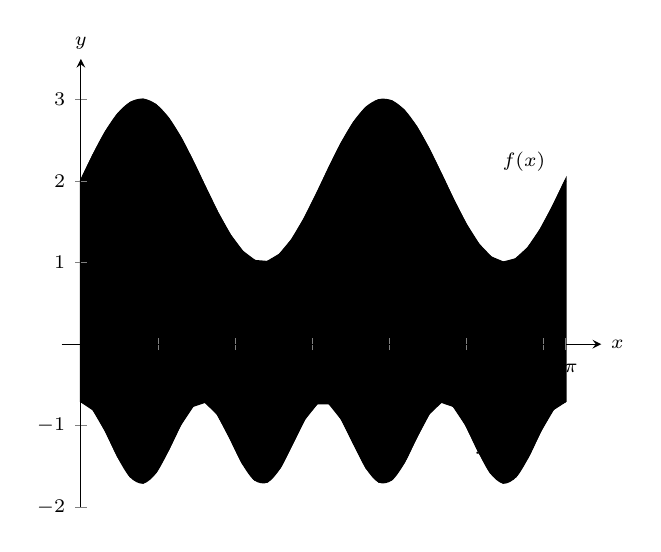
\begin{tikzpicture}
\begin{axis}[,%
tick label style={font=\scriptsize},axis y line=middle,axis x line=middle,name=myplot,axis on top,%
			%x=.37\marginparwidth,
			%y=.37\marginparwidth,
%			xtick=\empty,% 
			extra x ticks={12.57},
			extra x tick labels={$4\pi$},
%			ytick=\empty,
			%minor y tick num=1,%extra y ticks={-5,-3,...,7},%
%			minor x tick num=4,
			ymin=-2,ymax=3.5,%
			xmin=-.5,xmax=13.5%
]

\addplot [{\coloronefill},domain=0:12.57,stack plots=y,samples=40] {.5*cos(deg(2*x))-1.2};
\addplot [{\coloronefill},thick,fill={\coloronefill},area style,domain=0:12.57,stack plots=y,samples=40] {sin(deg(x))+2-(.5*cos(deg(2*x))-1.2)} \closedcycle;
\addplot [smooth,thick, {\colorone},domain=0:12.57,samples=40] {sin(deg(x))+2} node [shift={(-15pt,7pt)} ,black] {\scriptsize $f(x)$};
\addplot [smooth,thick, {\colorone},domain=0:12.57,samples=40] {.5*cos(deg(2*x))-1.2}node [shift={(-25pt,-16pt)} ,black] {\scriptsize $g(x)$};


\end{axis}

\node [right] at (myplot.right of origin) {\scriptsize $x$};
\node [above] at (myplot.above origin) {\scriptsize $y$};
\end{tikzpicture}}
}
\end{solution}


\begin{example}{Finding total area enclosed by curves}{ex_abc2}{
Find the total area of the region enclosed by the functions $f(x) = -2x+5$ and $g(x) = x^3-7x^2+12x-3$ as shown in Figure \ref{fig:abc2}.}
\end{example}

\begin{solution}
\begin{center}
\mfigure{.55}{Graphing a region enclosed by two functions in Example \ref{ex_abc2}.}{fig:abc2}{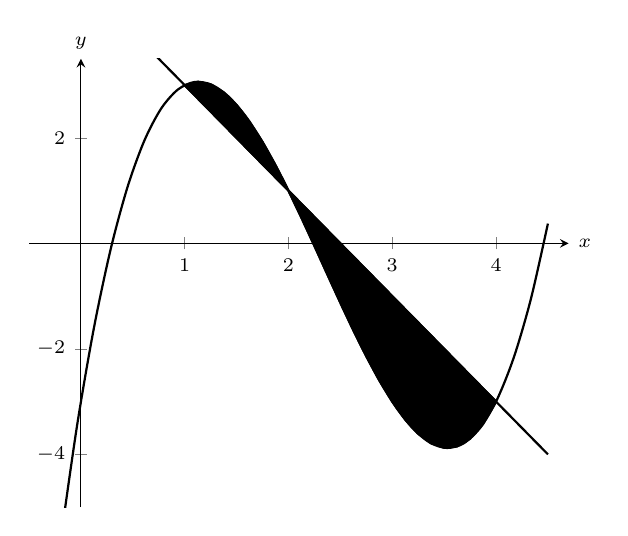
\begin{tikzpicture}
\begin{axis}[,%
tick label style={font=\scriptsize},axis y line=middle,axis x line=middle,name=myplot,axis on top,%
			%x=.37\marginparwidth,
			%y=.37\marginparwidth,
			xtick={1,2,3,4},% 
%			extra x ticks={12.57},
%			extra x tick labels={$4\pi$},
%			ytick=\empty,
			%minor y tick num=1,%extra y ticks={-5,-3,...,7},%
%			minor x tick num=4,
			ymin=-5,ymax=3.5,%
			xmin=-.5,xmax=4.7%
]

\addplot [{\coloronefill},stack plots=y,domain=1:4] {5-2*x};
\addplot [{\coloronefill},thick,fill={\coloronefill},area style,domain=1:4,stack plots=y] {x^3-7*x^2+12*x-3-(5-2*x)} \closedcycle;
\addplot [smooth,thick, {\colorone},domain=-.2:4.5,samples=30] {x^3-7*x^2+12*x-3};
\addplot [smooth,thick, {\colorone},domain=0:4.5] {5-2*x};


\end{axis}

\node [right] at (myplot.right of origin) {\scriptsize $x$};
\node [above] at (myplot.above origin) {\scriptsize $y$};
\end{tikzpicture}}
\end{center}

A quick calculation shows that $f=g$ at $x=1, 2$ and $ 4 $. One can proceed thoughtlessly by computing $\ds \int_1^4 \big(f(x)-g(x)\big)\ dx$, but this ignores the fact that on $[1,2]$, $g(x)>f(x)$. (In fact, the thoughtless integration returns $-9/4$, hardly the expected value of an \textit{area}.) Thus we compute the total area by breaking the interval $[1,4]$ into two subintervals, $[1,2]$ and $[2,4]$ and using the proper integrand in each.
\begin{align*}
\text{\mbox{\green{\bf Area}}} &= \int_1^4 \big|f(x)-g(x)\big|\ dx\\ 
&= \int_1^2 \big(g(x)-f(x)\big)\ dx + \int_2^4\big(f(x)-g(x)\big)\ dx\\
			&= \int_1^2 \big(x^3-7x^2+14x-8\big) \ dx + \int_2^4\big(-x^3+7x^2-14x+8\big)\ dx\\
			&= 5/12 + 8/3 \\
			&= 37/12 = 3.083\ \text{units}^2.
\end{align*}		
\end{solution}



The previous example makes note that we are expecting area to be \textit{positive}. When first learning about the definite integral, we interpreted it as ``signed area under the curve,'' allowing for ``negative area.'' That doesn't apply here; area is to be positive.

The previous example also demonstrates that we often have to break a given region into subregions before applying Theorem \ref{thm:areabetweencurves}. The following example shows another situation where this is applicable, along with an alternate view of applying the Theorem.\\


\begin{example}{Finding area: integrating with respect to $y$}{ex_abc3}
{
Find the area of the region enclosed by the functions $y=\sqrt{x}+2$, $y=-(x-1)^2+3$ and $y=2$, as shown in Figure \ref{fig:abc3}.}
\end{example}



\begin{solution}
{We give two approaches to this problem. In the first approach, we notice that the region's ``top'' is defined by two different curves. On $[0,1]$, the top function is $y=\sqrt{x}+2$; on $[1,2]$, the top function is $y=-(x-1)^2+3$. 

\begin{center}
\mfigure{.55}{Graphing a region for Example \ref{exa:ex_abc3}.}{fig:abc3}{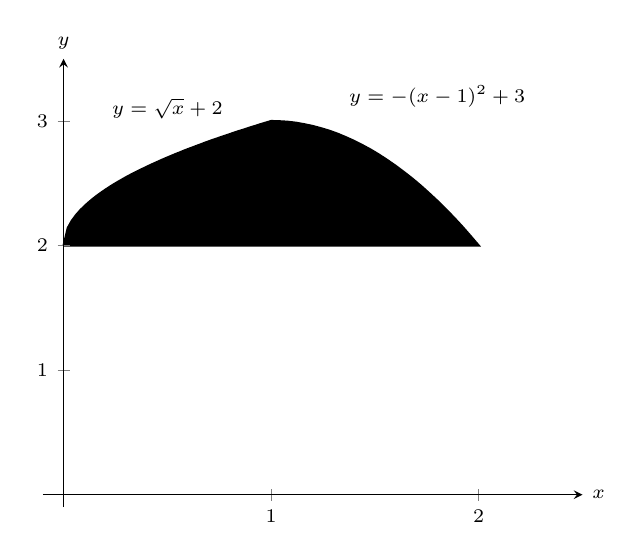
\begin{tikzpicture}
\begin{axis}[,%
tick label style={font=\scriptsize},axis y line=middle,axis x line=middle,name=myplot,axis on top,%
			%x=.37\marginparwidth,
			%y=.37\marginparwidth,
			xtick={1,2},% 
%			extra x ticks={12.57},
%			extra x tick labels={$4\pi$},
%			ytick=\empty,
			%minor y tick num=1,%extra y ticks={-5,-3,...,7},%
%			minor x tick num=4,
			ymin=-.1,ymax=3.5,%
			xmin=-.1,xmax=2.5%
]

\addplot [{\colorone},thick,fill={\coloronefill}] coordinates {(0,2.)(0.02,2.141)(0.04,2.2)(0.06,2.245)(0.08,2.283)(0.1,2.316)(0.12,2.346)(0.14,2.374)(0.16,2.4)(0.18,2.424)(0.2,2.447)(0.22,2.469)(0.24,2.49)(0.26,2.51)(0.28,2.529)(0.3,2.548)(0.32,2.566)(0.34,2.583)(0.36,2.6)(0.38,2.616)(0.4,2.632)(0.42,2.648)(0.44,2.663)(0.46,2.678)(0.48,2.693)(0.5,2.707)(0.52,2.721)(0.54,2.735)(0.56,2.748)(0.58,2.762)(0.6,2.775)(0.62,2.787)(0.64,2.8)(0.66,2.812)(0.68,2.825)(0.7,2.837)(0.72,2.849)(0.74,2.86)(0.76,2.872)(0.78,2.883)(0.8,2.894)(0.82,2.906)(0.84,2.917)(0.86,2.927)(0.88,2.938)(0.9,2.949)(0.92,2.959)(0.94,2.97)(0.96,2.98)(0.98,2.99)(1.,3.)(1.04,2.998)(1.08,2.994)(1.12,2.986)(1.16,2.974)(1.2,2.96)(1.24,2.942)(1.28,2.922)(1.32,2.898)(1.36,2.87)(1.4,2.84)(1.44,2.806)(1.48,2.77)(1.52,2.73)(1.56,2.686)(1.6,2.64)(1.64,2.59)(1.68,2.538)(1.72,2.482)(1.76,2.422)(1.8,2.36)(1.84,2.294)(1.88,2.226)(1.92,2.154)(1.96,2.078)(2.,2.)(0,2)};

\draw (axis cs:.5,3.1) node {\scriptsize $y=\sqrt{x}+2$} (axis cs:1.8,3.2) node {\scriptsize $y=-(x-1)^2+3$};

\end{axis}

\node [right] at (myplot.right of origin) {\scriptsize $x$};
\node [above] at (myplot.above origin) {\scriptsize $y$};
\end{tikzpicture}}
\end{center}

Thus we compute the area as the sum of two integrals:
\begin{align*}
\mbox{\green{\bf Area}} &= \int_0^1 \Big(\big(\sqrt{x}+2\big)-2\Big)\ dx + \int_1^2 \Big(\big(-(x-1)^2+3\big)-2\Big)\ dx \\
									&= 2/3 + 2/3\\
									&=4/3.
\end{align*}

The second approach is clever and very useful in certain situations. We are used to viewing curves as functions of $x$; we input an $x$-value and a $y$-value is returned. Some curves can also be described as functions of $y$: input a $y$-value and an $x$-value is returned. We can rewrite the equations describing the boundary by solving for $x$:
	$$y=\sqrt{x}+2 \quad \Rightarrow\quad x=(y-2)^2$$
	$$y=-(x-1)^2+3 \quad \Rightarrow \quad x=\sqrt{3-y}+1.$$

\mfigure{.8}{The region used in Example \ref{ex_abc3} with boundaries relabeled as functions of $y$.}{fig:abc3b}{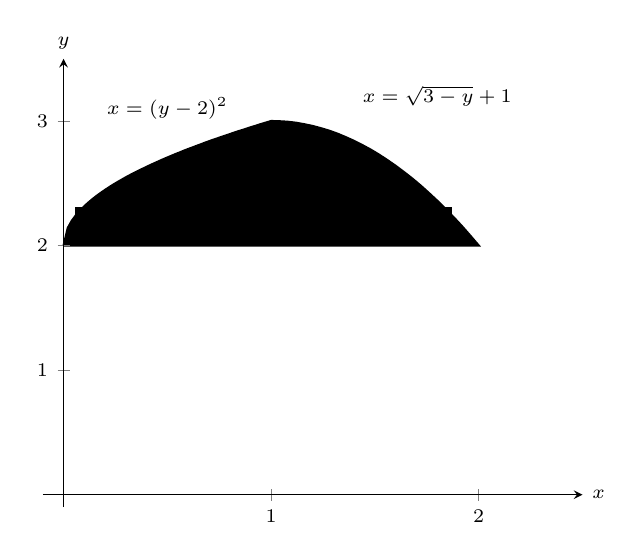
\begin{tikzpicture}
\begin{axis}[,%
tick label style={font=\scriptsize},axis y line=middle,axis x line=middle,name=myplot,axis on top,%
			%x=.37\marginparwidth,
			%y=.37\marginparwidth,
			xtick={1,2},% 
%			extra x ticks={12.57},
%			extra x tick labels={$4\pi$},
%			ytick=\empty,
			%minor y tick num=1,%extra y ticks={-5,-3,...,7},%
%			minor x tick num=4,
			ymin=-.1,ymax=3.5,%
			xmin=-.1,xmax=2.5%
]

\addplot [{\colorone},thick,fill={\coloronefill}] coordinates {(0,2.)(0.02,2.141)(0.04,2.2)(0.06,2.245)(0.08,2.283)(0.1,2.316)(0.12,2.346)(0.14,2.374)(0.16,2.4)(0.18,2.424)(0.2,2.447)(0.22,2.469)(0.24,2.49)(0.26,2.51)(0.28,2.529)(0.3,2.548)(0.32,2.566)(0.34,2.583)(0.36,2.6)(0.38,2.616)(0.4,2.632)(0.42,2.648)(0.44,2.663)(0.46,2.678)(0.48,2.693)(0.5,2.707)(0.52,2.721)(0.54,2.735)(0.56,2.748)(0.58,2.762)(0.6,2.775)(0.62,2.787)(0.64,2.8)(0.66,2.812)(0.68,2.825)(0.7,2.837)(0.72,2.849)(0.74,2.86)(0.76,2.872)(0.78,2.883)(0.8,2.894)(0.82,2.906)(0.84,2.917)(0.86,2.927)(0.88,2.938)(0.9,2.949)(0.92,2.959)(0.94,2.97)(0.96,2.98)(0.98,2.99)(1.,3.)(1.04,2.998)(1.08,2.994)(1.12,2.986)(1.16,2.974)(1.2,2.96)(1.24,2.942)(1.28,2.922)(1.32,2.898)(1.36,2.87)(1.4,2.84)(1.44,2.806)(1.48,2.77)(1.52,2.73)(1.56,2.686)(1.6,2.64)(1.64,2.59)(1.68,2.538)(1.72,2.482)(1.76,2.422)(1.8,2.36)(1.84,2.294)(1.88,2.226)(1.92,2.154)(1.96,2.078)(2.,2.)(0,2)};

\draw (axis cs:.5,3.1) node {\scriptsize $x=(y-2)^2$} (axis cs:1.8,3.2) node {\scriptsize $x=\sqrt{3-y}+1$};

\filldraw [{\colortwo},fill={\colortwofill},thick] (axis cs: 0.0625,2.2) rectangle (axis cs:1.867,2.3);

\end{axis}

\node [right] at (myplot.right of origin) {\scriptsize $x$};
\node [above] at (myplot.above origin) {\scriptsize $y$};
\end{tikzpicture}}	

Figure \ref{fig:abc3b} shows the region with the boundaries relabeled. A differential element, a horizontal rectangle, is also pictured.	The width of the rectangle is a small change in $y$: $\Delta y$. The height of the rectangle is a difference in $x$-values. The ``top'' $x$-value is the largest value, i.e., the rightmost. The ``bottom'' $x$-value is the smaller, i.e., the leftmost. Therefore the height of the rectangle is $$\big(\sqrt{3-y}+1\big) - (y-2)^2.$$

The area is found by integrating the above function with respect to $y$ with the appropriate bounds. We determine these by considering the $y$-values the region occupies. It is bounded below by $y=2$, and bounded above by $y=3$. That is, both the ``top'' and ``bottom'' functions exist on the $y$ interval $[2,3]$. Thus
\begin{align*}
\mbox{\green{\bf Area}} &= \int_2^3 \big(\sqrt{3-y}+1 - (y-2)^2\big)\ dy \\
			&= \Big(-\frac23(3-y)^{3/2}+y-\frac13(y-2)^3\Big)\Big|_2^3 \\
			&= 4/3.
\end{align*}
\vskip-\baselineskip
}
\end{solution}


Sometimes the given curves are not given as functions of $x$, but rather functions of $ y $.
In this instances, it may be more useful to use the "horizontal rectangle" approach outlined above.
$$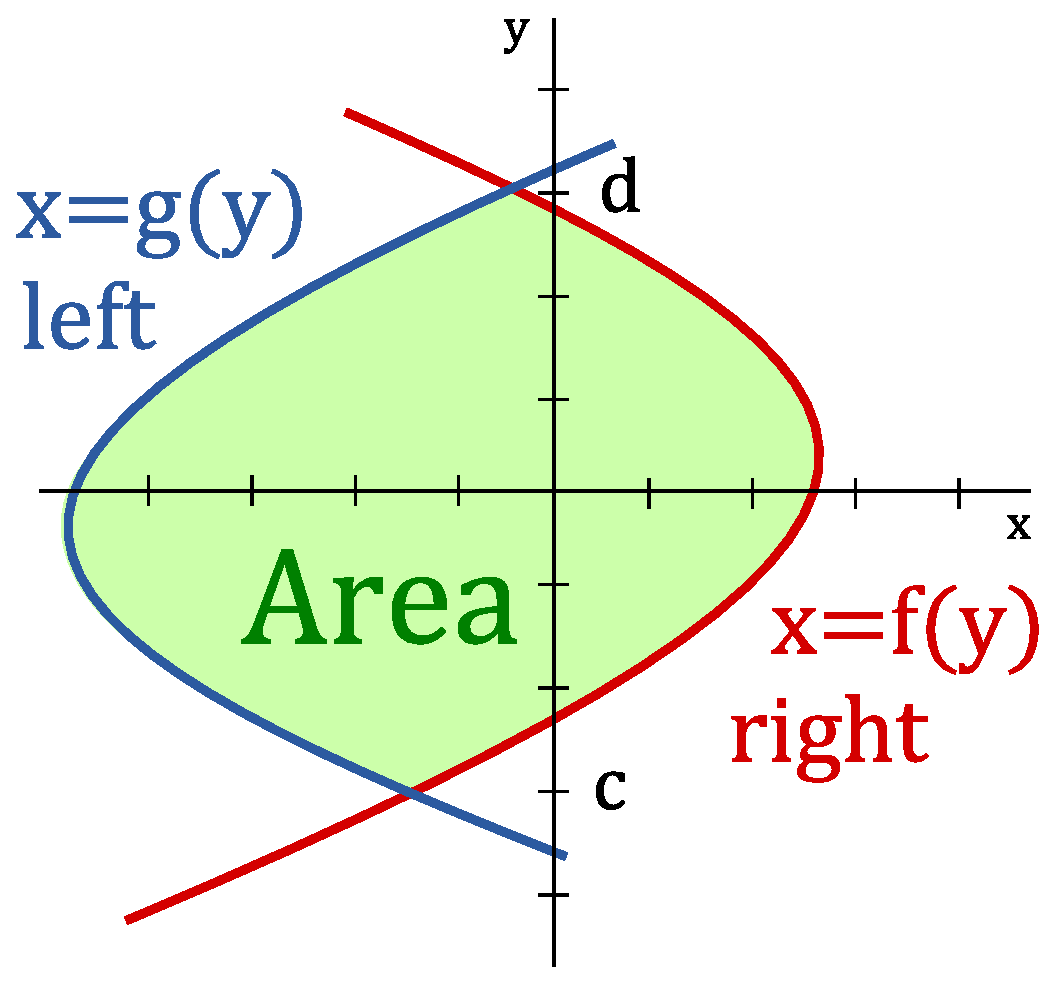
\includegraphics[width=2.5in]{images2/area-between-formula-2}$$
The area $A$ of the region bounded by the curves $x=f(y)$ and $x=g(y)$ and the lines $y=c$ and $y=d$ is:
$$A=\int_c^d\left|f(y)-g(y)\right|\,dy.$$ 
Informally this can be thought of as follows:

\begin{formulabox}[Area Between Two Curves]
$$Area=\int_c^d (\mbox{right curve}) - (\mbox{left curve})\,dy,\qquad c\leq y\leq d.$$
\end{formulabox}
 
\begin{example}{Area Between Two Curves}{Area Between Two Curves}
Determine the area enclosed by $x=y^2$ and $x=8$.
\end{example} 

\begin{solution}
Note that $x=y^2$ and $x=8$ intersect when:  
$$y^2=8\qquad\to  \qquad y=\pm\sqrt 8\qquad\to \qquad y=\pm 2\sqrt 2$$ 
Sketching the two curves gives:

$$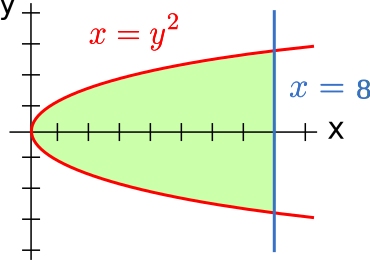
\includegraphics[width=2.5in]{images2/area-between-example-3}$$


From the sketch $c=-2\sqrt 2$, $d=2\sqrt 2$, the right curve is $x=8$ and the left curve is $x=y^2$.
$$\mbox{\exfont{Area}}
~=~\int_c^d[\mbox{right}-\mbox{left}]\,dy
~=~\int_{-2\sqrt 2}^{2\sqrt 2} (8-y^2)\,dy 
~=~\left.\left(8y-\frac{1}{3}y^3\right)\right|_{-2\sqrt 2}^{2\sqrt 2}$$ 
$$= \left[8(2\sqrt 2)-\frac{1}{3}(2\sqrt 2)^3\right] - \left[8(-2\sqrt 2)-\frac{1}{3}(-2\sqrt 2)^3\right]
~=~\frac{64\sqrt 2}{3}$$
\end{solution}


























\begin{example}{Area Between Two Curves}{Area Between Two Curves}
Determine the area enclosed by $y=x^2$, $y=\sqrt x$, $x=0$ and $x=2$.
\end{example} 

\begin{solution}
The points of intersection of $y=x^2$ and $y=\sqrt x$ are
$$x^2=\sqrt x\qquad\to \qquad x^4=x\qquad\to \qquad x^4-x=0 \qquad\to \qquad x(x^3-1)=0.$$
Thus, either $x=0$ or $x=1$.
Sketching the curves gives:

\begin{tikzpicture} %[scale=.6]
\begin{axis}[
        xmin=-1,
        xmax=2.5,
        ymin=-1,
        ymax=4.5,
       % y=2cm,
       % x=1cm,
    domain=-0.2:2.1,
    samples=40,
    axis lines=middle,
   % xtick = {0.78539, 1.57079, 2.3561,3.1415, 3.92699,4.7123,5.49778,6.28318,7.06858},
 % xticklabels = {$\frac{\pi}{4}$,$\frac{\pi}{2}$,$\frac{3\pi}{4}$,$\pi $, $\frac{5\pi}{4}$, $\frac{3\pi}{2}$, $\frac{7\pi}{4}$, $2\pi$,},
 %   ytick={-1,1},
]
\addplot [ thick, red,name path=A] {x^2}; 
\draw[red] (axis cs:1.5,4) node {$y=x^2$};
\addplot [thick, blue,name path=B,domain=0:2.1] {sqrt(x)};
\draw[blue] (axis cs:1.6,.8) node {$y=\sqrt{x}$};
\draw[blue] (axis cs: .4,.4) node {\scriptsize $A_1$};
\draw[blue] (axis cs:1.6,1.8) node {\scriptsize $A_2$};
% \addplot [draw=none,name path=B] {0};     % “fictional” curve
  \addplot [\coloronefill] fill between[of = A and B,soft clip={domain=0:2}]; % filling
\end{axis}
\end{tikzpicture}


%$$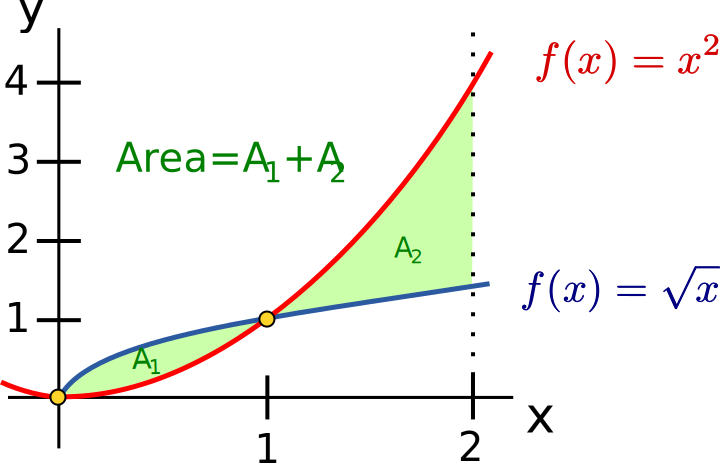
\includegraphics[width=2.75in]{images2/area-between-example-2}$$
The area we want to compute is the shaded region. 
Since the top curve changes at $x=1$, we need to use the formula twice. 
For $A_1$ we have $a=0$, $b=1$, the top curve is $y=\sqrt x$ and the bottom curve is $y=x^2$. 
For $A_2$ we have $a=1$, $b=2$, the top curve is $y=x^2$ and the bottom curve is $y=\sqrt x$. 
$$\mbox{\green{\bf Area}}
~=~\mbox{\green{\bf A$_1$}}+\mbox{\green{\bf A$_2$}}  
~=~\int_0^1(\sqrt x-x^2)\,dx+\int_1^2(x^2-\sqrt x)\,dx$$
For the first integral we have:
$$\int_0^1(\sqrt x-x^2)\,dx  
~=~\left.\left(\frac{2}{3}x^{3/2}-\frac{1}{3}x^3\right)\right|_0^1  
~=~\frac{1}{3}$$
Thus,
$$\mbox{\green{\bf Area}}~=~\frac{1}{3}+\left.\left(\frac{1}{3}x^3-\frac{2}{3}x^{3/2}\right)\right|_1^2 
~=~\frac{1}{3}+\left[\left(\frac{8}{3}-\frac{2(\sqrt 2)^3}{3}\right)-\left(\frac{1}{3}-\frac{2}{3}\right)\right] 
~=~\frac{10-4\sqrt 2}{3}$$
\end{solution}

\begin{example}{Area Between Sine and Cosine}{Area Between Sine and Cosine}
Determine the area enclosed by $y=\sin x$ and $y=\cos x$ on the interval $[0,~2\pi]$.
\end{example}

\begin{solution}
The curves $y=\sin x$ and $y=\cos x$ intersect when:  
$$\sin x=\cos x\qquad\to  \qquad \tan x = 1\qquad\to  \qquad x=\frac{\pi}{4}+\pi k,~\mbox{$k$ an integer.}$$
We have the following sketch:




\begin{tikzpicture} %[scale=.6]
\begin{axis}[
        xmin=-1.5,
        xmax=8,
        ymin=-1.5,
        ymax=1.5,
        y=3cm/2,
        x=1.7cm,
    domain=0:5*pi/2,
    samples=100,
    axis lines=middle,
    xtick = {0.78539, 1.57079, 2.3561,3.1415, 3.92699,4.7123,5.49778,6.28318,7.06858
    },
  xticklabels = {$\frac{\pi}{4}$,$\frac{\pi}{2}$,$\frac{3\pi}{4}$,$\pi $, $\frac{5\pi}{4}$, $\frac{3\pi}{2}$, $\frac{7\pi}{4}$, $2\pi$,},
    ytick={-1,1},
]
\addplot [samples=501,mark=none, thick, red,name path=A,domain=-2*pi:3*pi] {cos(deg(x))}; \draw[red] (axis cs:-1,1) node {$\cos(x)$};
\addplot [samples=501,mark=none, thick, blue,name path=B,domain=-2*pi:3*pi] {sin(deg(x))};
\draw[blue] (axis cs:-1,-.4) node {$\sin(x)$};
% \addplot [draw=none,name path=B] {0};     % “fictional” curve
  \addplot [\coloronefill] fill between[of = A and B,soft clip={domain=0:2*pi}]; % filling
\end{axis}
\end{tikzpicture}


%$$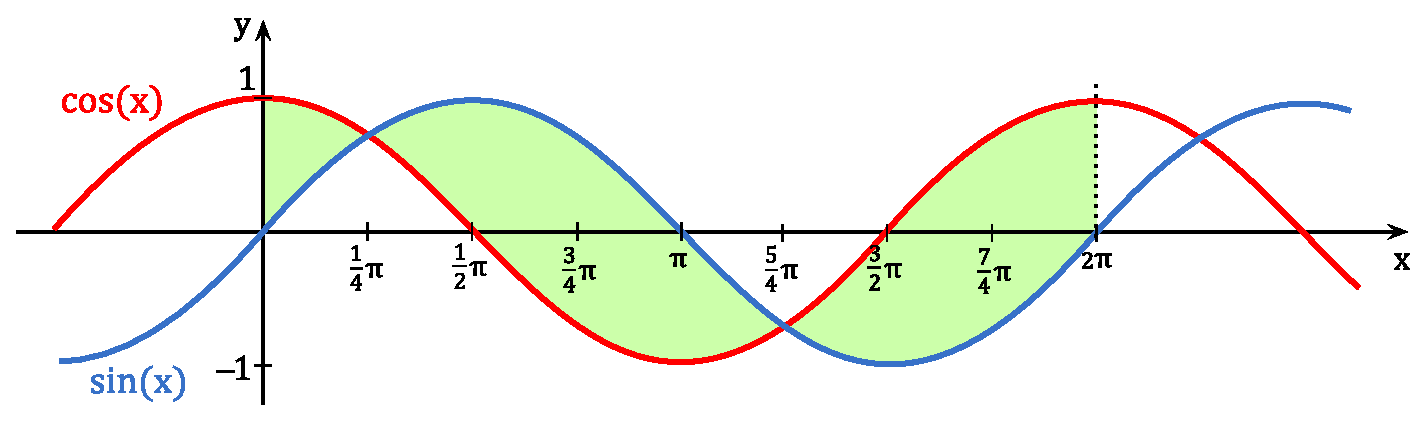
\includegraphics[width=5.5in]{images2/area-between-example-4}$$
The area we want to compute is the shaded region.
The top curve changes at $x=\pi/4$ and $x=5\pi/4$, thus, we need to split the area up into three regions:
from $0$ to $\pi/4$; from $\pi/4$ to $5\pi/4$; and from $5\pi/4$ to $2\pi$. 
\begin{eqnarray*}
\mbox{\green{\bf Area}} & = & \int_0^{\frac{\pi}{4}}(\cos x-\sin x)\,dx  + \int_{\frac{\pi}{4}}^{\frac{5\pi}{4}}(\sin x-\cos x)\,dx  + \int_{\frac{5\pi}{4}}^{2\pi}(\cos x-\sin x)\,dx\\  
			 & = & \left(\sin x + \cos x\right)\bigg|_0^{\pi/4}+ \left(-\cos x - \sin x\right)\bigg|_{\pi/4}^{5\pi/4} +  \left(\sin x + \cos x\right)\bigg|_{5\pi/4}^{2\pi}\\ 
			& = & \left(\sqrt 2-1\right) + \left(\sqrt 2+\sqrt 2\right) + \left(1+\sqrt 2\right)\\ 
			& = & 4\sqrt 2
\end{eqnarray*}
\end{solution}





%
This calculus--based technique of finding area can be useful even with shapes that we normally think of as ``easy.'' Example \ref{ex_abc4} computes the area of a triangle. While the formula ``$\frac12\times\text{base}\times\text{height}$'' is well known, in arbitrary triangles it can be nontrivial to compute the height. Calculus makes the problem simple.\\

\begin{example}{Finding the area of a triangle}{ex_abc4}
{
Compute the area of the regions bounded by the lines  $y=x+1$, $y=-2x+7$ and $y=-\frac12x+\frac52$, as shown in Figure \ref{fig:abc4}.}
\end{example}


\begin{solution}
{Recognize that there are two ``top'' functions to this region, causing us to use two definite integrals.
\begin{align*}
\text{Total Area} &= \int_1^2\big((x+1)-(-\frac12x+\frac52)\big)\ dx + \int_2^3\big((-2x+7)-(-\frac12x+\frac52)\big)\ dx \\
						&= 3/4+3/4\\
						&=3/2.
\end{align*}

\mfigure{.8}{Graphing a triangular region in Example \ref{ex_abc4}.}{fig:abc4}{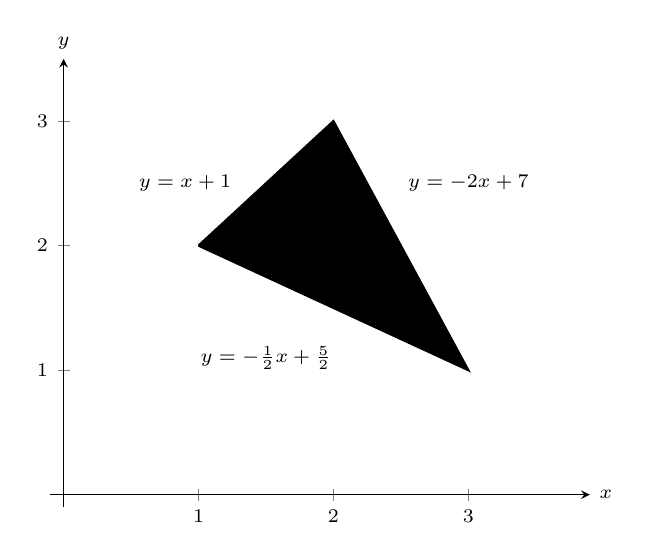
\begin{tikzpicture}
\begin{axis}[ %width=\marginparwidth+25pt,%
tick label style={font=\scriptsize},axis y line=middle,axis x line=middle,name=myplot,axis on top,%
			%x=.37\marginparwidth,
			%y=.37\marginparwidth,
			xtick={1,2,3},% 
%			extra x ticks={12.57},
%			extra x tick labels={$4\pi$},
%			ytick=\empty,
			%minor y tick num=1,%extra y ticks={-5,-3,...,7},%
%			minor x tick num=4,
			ymin=-.1,ymax=3.5,%
			xmin=-.1,xmax=3.9%
]

\addplot [{\colorone},thick,fill={\coloronefill}] coordinates {(1,2) (2,3) (3,1) (1,2)};

\draw (axis cs:.9,2.5) node {\scriptsize $y=x+1$} (axis cs:3,2.5) node {\scriptsize $y=-2x+7$} (axis cs:1.5,1.1) node {\scriptsize $y=-\frac12x+\frac52$};
%
%\filldraw [{\colortwo},fill={\colortwofill},thick] (axis cs: 0.0625,2.2) rectangle (axis cs:1.867,2.3);

\end{axis}

\node [right] at (myplot.right of origin) {\scriptsize $x$};
\node [above] at (myplot.above origin) {\scriptsize $y$};
\end{tikzpicture}}

We can also approach this by converting each function into a function of $y$. This also requires $ 2 $ integrals, so there isn't really any advantage to doing so. We do it here for demonstration purposes.

The ``top'' function is always $x=\frac{7-y}2$ while there are two ``bottom'' functions. Being mindful of the proper integration bounds, we have
\begin{align*}
\text{Total Area} &= \int_1^2\big(\frac{7-y}2 - (5-2y)\big)\ dy + \int_2^3\big(\frac{7-y}2-(y-1)\big)\ dy \\
			&= 3/4 + 3/4\\
			&= 3/2.
\end{align*}
Of course, the final answer is the same. (It is interesting to note that the area of all 4 subregions used is 3/4. This is coincidental.)
}
\end{solution}


%
While we have focused on producing exact answers, we are also able to make approximations using the principle of Theorem \ref{thm:areabetweencurves}. The integrand in the theorem is a distance (``top minus bottom''); integrating this distance function gives an area. By taking discrete measurements of distance, we can approximate an area using numerical integration techniques developed in Section \ref{sec:numerical_integration}. The following example demonstrates this.\\

\begin{example}{Numerically approximating area}{ex_abc5}{
To approximate the area of a lake, shown in Figure \ref{fig:abc5} (a),  the ``length'' of the lake is measured at $ 200 $-meter increments as shown in Figure \ref{fig:abc5} (b), where the lengths are given in hundreds of meters. Approximate the area of the lake.}
\end{example}


\begin{solution}
{The measurements of length can be viewed as measuring ``top minus bottom'' of two functions. The exact answer is found by integrating $\ds \int_0^{12} \big(f(x)-g(x)\big)\ dx$, but of course we don't know the functions $f$ and $g$. Our discrete measurements instead allow us to approximate.


\begin{figure}[H]
	\centering
	\begin{subfigure}[t]{0.5\textwidth}
             {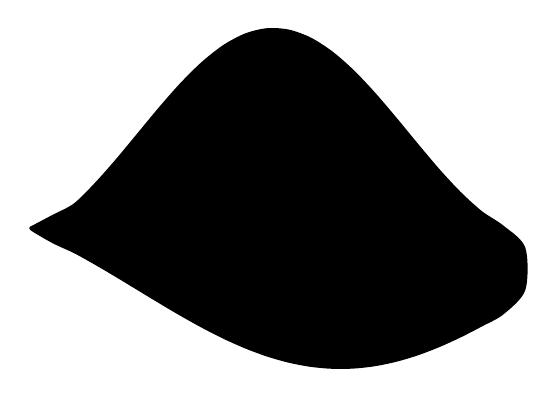
\begin{tikzpicture}
                 		\begin{axis}[ %width=\marginparwidth+25pt,%
                 		tick label style={font=\scriptsize},axis lines=none,name=myplot,%
                 					%x=.37\marginparwidth,
                 					%y=.37\marginparwidth,
                 		%			xtick={1,2,3,4,5,6,7,8,9,10,11,12},% 
                 		%			extra x ticks={12.57},
                 		%			extra x tick labels={$4\pi$},
                 		%			ytick={1,2,3,4,5,6,7,8},
                 					%minor y tick num=1,%extra y ticks={-5,-3,...,7},%
                 		%			minor x tick num=4,
                 					ymin=-.1,ymax=8.5,%
                 					xmin=-.1,xmax=12.5%
                 		]
                 		
                 		\addplot [{\colorone},thick,fill={\coloronefill},smooth] coordinates {(0,3.2)(0.5,3.417)(1.,3.637)(1.5,4.041)(2.,4.505)(2.5,5.)(3.,5.495)(3.5,5.959)(4.,6.363)(4.5,6.683)(5.,6.898)(5.5,6.995)(6.,6.968)(6.5,6.819)(7.,6.556)(7.5,6.197)(8.,5.763)(8.5,5.282)(9.,4.784)(9.5,4.298)(10.,3.857)(10.5,3.486)(11.,3.21)(11.5,2.8)(11.5,2)(11.,1.545)(10.5,1.314)(10.,1.102)(9.5,0.9154)(9.,0.7585)(8.5,0.6361)(8.,0.5514)(7.5,0.5069)(7.,0.5038)(6.5,0.5421)(6.,0.6208)(5.5,0.7378)(5.,0.8897)(4.5,1.072)(4.,1.281)(3.5,1.509)(3.,1.751)(2.5,2.)(2.,2.249)(1.5,2.491)(1.,2.719)(0.5,2.9102)(0,3.15)(0,3.2)};
                 		%(0.5,3.317)
%                 		\draw (axis cs:2,4.5) -- (axis cs:2,2.249) node [shift={(-3pt,0pt)},rotate=90,pos=.5] {\scriptsize 2.25}
%                 		(axis cs:4,6.36) -- (axis cs:4,1.28) node [shift={(-3pt,0pt)},rotate=90,pos=.5] {\scriptsize 5.08}
%                 		(axis cs:6,6.97) -- (axis cs:6,0.62) node [shift={(-3pt,0pt)},rotate=90,pos=.5] {\scriptsize 6.35}
%                 		(axis cs:8,5.76) -- (axis cs:8,.55) node  [shift={(-3pt,0pt)},rotate=90,pos=.5] {\scriptsize 5.21}
%                 		(axis cs:10,3.86) -- (axis cs:10,1.1) node [shift={(-3pt,0pt)},rotate=90,pos=.5] {\scriptsize 2.76};
                 		\end{axis}
                 		
%                 		\node [right] at (myplot.right of origin) {\scriptsize $x$};
%                 		\node [above] at (myplot.above origin) {\scriptsize $y$};
                 		\end{tikzpicture}}	
        \label{fig:abc5a}
        \caption{A sketch of a lake.} 
    \end{subfigure}% 
    \begin{subfigure}[t]{0.5\textwidth}
    {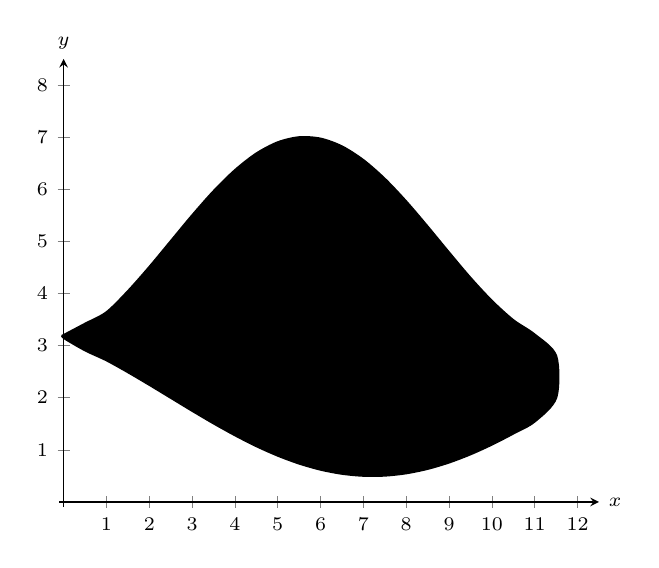
\begin{tikzpicture}
    		\begin{axis}[ %width=\marginparwidth+25pt,%
    		tick label style={font=\scriptsize},axis y line=middle,axis x line=middle,name=myplot,axis on top,%
    					%x=.37\marginparwidth,
    					%y=.37\marginparwidth,
    					xtick={1,2,3,4,5,6,7,8,9,10,11,12},% 
    		%			extra x ticks={12.57},
    		%			extra x tick labels={$4\pi$},
    					ytick={1,2,3,4,5,6,7,8},
    					%minor y tick num=1,%extra y ticks={-5,-3,...,7},%
    		%			minor x tick num=4,
    					ymin=-.1,ymax=8.5,%
    					xmin=-.1,xmax=12.5%
    		]
    		
    		\addplot [{\colorone},thick,fill={\coloronefill},smooth] coordinates {(0,3.2)(0.5,3.417)(1.,3.637)(1.5,4.041)(2.,4.505)(2.5,5.)(3.,5.495)(3.5,5.959)(4.,6.363)(4.5,6.683)(5.,6.898)(5.5,6.995)(6.,6.968)(6.5,6.819)(7.,6.556)(7.5,6.197)(8.,5.763)(8.5,5.282)(9.,4.784)(9.5,4.298)(10.,3.857)(10.5,3.486)(11.,3.21)(11.5,2.8)(11.5,2)(11.,1.545)(10.5,1.314)(10.,1.102)(9.5,0.9154)(9.,0.7585)(8.5,0.6361)(8.,0.5514)(7.5,0.5069)(7.,0.5038)(6.5,0.5421)(6.,0.6208)(5.5,0.7378)(5.,0.8897)(4.5,1.072)(4.,1.281)(3.5,1.509)(3.,1.751)(2.5,2.)(2.,2.249)(1.5,2.491)(1.,2.719)(0.5,2.9102)(0,3.15)(0,3.2)};
    		%(0.5,3.317)
    		\draw (axis cs:2,4.5) -- (axis cs:2,2.249) node [shift={(-3pt,0pt)},rotate=90,pos=.5] {\scriptsize 2.25}
    		(axis cs:4,6.36) -- (axis cs:4,1.28) node [shift={(-3pt,0pt)},rotate=90,pos=.5] {\scriptsize 5.08}
    		(axis cs:6,6.97) -- (axis cs:6,0.62) node [shift={(-3pt,0pt)},rotate=90,pos=.5] {\scriptsize 6.35}
    		(axis cs:8,5.76) -- (axis cs:8,.55) node  [shift={(-3pt,0pt)},rotate=90,pos=.5] {\scriptsize 5.21}
    		(axis cs:10,3.86) -- (axis cs:10,1.1) node [shift={(-3pt,0pt)},rotate=90,pos=.5] {\scriptsize 2.76};
    		
    		
    		\end{axis}
    		
    		\node [right] at (myplot.right of origin) {\scriptsize $x$};
    		\node [above] at (myplot.above origin) {\scriptsize $y$};
    		\end{tikzpicture}}

        \label{fig:abc5b}
        \caption{The lake with length measurements.}    
    \end{subfigure} 
    \caption{\label{fig:abc5}}
\end{figure}



We have the following data points:
$$(0,0),\ (2,2.25),\ (4,5.08),\ (6,6.35),\ (8,5.21),\ (10,2.76),\ (12,0).$$
We also have that $\dx=\frac{b-a}{n} = 2$, so Simpson's Rule gives
\begin{align*}
\text{Area}&\approx \frac{2}{3}\Big(1\cdot0+4\cdot2.25+2\cdot5.08+4\cdot6.35+2\cdot5.21+4\cdot2.76+1\cdot0\Big)\\
			&= 44.01\overline{3} \ \text{100m.}^2.
\end{align*}

Since the measurements are in hundreds of meters, units$^2 = (100\ \text{m})^2 = 10,000\ \text{m}^2$, giving a total area of $440,133\ \text{m}^2$. (Since we are approximating, we'd likely say the area was about $440,000\ \text{m}^2$, which is   $ 44 $ hectares.)
}
\end{solution}




In the next section we apply our applications--of--integration techniques to finding the volumes of certain solids.
































%% % % % % % % % % % % % % % % % % % % % % % % % % % % % % % % % % % % % % % % % % % % % % % % % % % % % % % % % % % % % %
%
%We have seen how integration can be used to find an area between a
%curve and the $x$-axis. With very little change we can find some areas
%between curves; indeed, the area between a curve and the $x$-axis may
%be interpreted as the area between the curve and a second ``curve''
%with equation $y=0$. 
%%In the simplest of cases, the idea is quite easy to understand.
%
%%\begin{example}{Area between Curves} {AreaBetweenCurves} 
%%Find the area below $\ds f(x)= -x^2+4x+3$ and above
%%$\ds g(x)=-x^3+7x^2-10x+5$ over the interval $1\le x\le2$. 
%%\end{example}
%%
%%\begin{solution} 
%%In the figure below we show the two curves together, with
%%the desired area shaded, then $f$ alone with the area under $f$
%%shaded, and then $g$ alone with the area under $g$ shaded. 
%%
%%\[
%%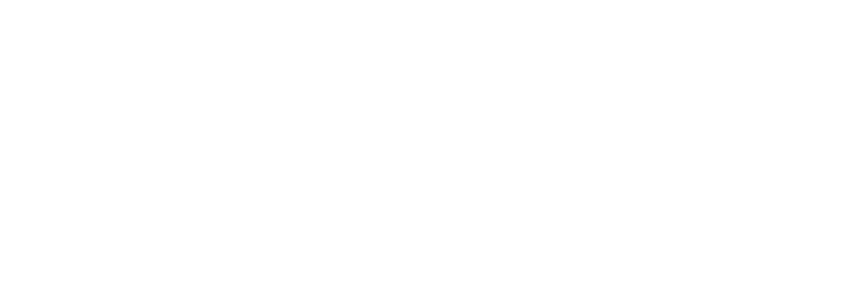
\includegraphics[width=5in]{images/area-between1} 
%%\]
%%%\figure[!ht]
%%%\hbox to \hsize{\hfill
%%%\def\yarrow{-- +(-1.5pt,-3pt) +(0pt,0pt) -- +(1.5pt,-3pt) +(0pt,0pt)}
%%%\def\xarrow{-- +(-3pt,-1.5pt) +(0pt,0pt) -- +(-3pt,1.5pt) +(0pt,0pt) }
%%%\tikzpicture[domain=0:3,y=3mm]
%%%\draw[->] (0,0) -- (3.2,0) \xarrow node [right] {$x$};
%%%\draw[->] (0,0) -- (0,11.2) \yarrow node [above] {$y$};
%%%\gpad
%%%\draw[color=black] plot[id=\the\gpnum,domain=0:3] function{-x**3+7*x**2-10*x+5};
%%%\gpad
%%%\draw[color=black] plot[id=\the\gpnum,domain=0:3] function{-x**2+4*x+3};
%%%\draw[dashed] (1,0) -- (1,6);
%%%\draw[dashed] (2,0) -- (2,7);
%%%\foreach \x in {0,1,2,3} \draw (\x,0) -- (\x,-2pt) node[anchor=north] {$\x$};
%%%\foreach \y in {0,5,10} \draw (0,\y) -- (-2pt,\y) node[anchor=east]
%%%         {$\y$};
%%%\gpad
%%%\fill[opacity=0.5,fill=red!20] plot[id=\the\gpnum,domain=1:2]
%%%function{-x**3+7*x**2-10*x+5} -- (2,7) node {\gpad}
%%%plot[parametric,id=\the\gpnum,domain=0:1] function{2-t,-t**2+7} -- (1,1);
%%%\endtikzpicture
%%% 
%%%\tikzpicture[domain=0:3,y=3mm]
%%%\draw[->] (0,0) -- (3.2,0) \xarrow node [right] {$x$};
%%%\draw[->] (0,0) -- (0,11.2) \yarrow node [above] {$y$};
%%%\gpad
%%%\draw[color=black] plot[id=\the\gpnum,domain=0:3] function{-x**2+4*x+3};
%%%\draw[dashed] (1,0) -- (1,6);
%%%\draw[dashed] (2,0) -- (2,7);
%%%\foreach \x in {0,1,2,3} \draw (\x,0) -- (\x,-2pt) node[anchor=north] {$\x$};
%%%\foreach \y in {0,5,10} \draw (0,\y) -- (-2pt,\y) node[anchor=east] {$\y$};
%%%\gpad\fill[opacity=0.5,fill=red!20] (2,0) -- (2,7)
%%%plot[parametric,id=\the\gpnum,domain=0:1] function{2-t,-t**2+7} -- (1,0) -- (2,0);
%%%\endtikzpicture
%%%
%%%\tikzpicture[domain=0:3,y=3mm]
%%%\draw[angle 90] (0,0) -- (3.2,0) \xarrow node [right] {$x$};
%%%\draw[->] (0,0) -- (0,11.2) \yarrow node [above] {$y$};
%%%\gpad\draw[color=black] plot[id=\the\gpnum,domain=0:3] function{-x**3+7*x**2-10*x+5};
%%%\draw[dashed] (1,0) -- (1,1);
%%%\draw[dashed] (2,0) -- (2,5);
%%%\foreach \x in {0,1,2,3} \draw (\x,0) -- (\x,-2pt) node[anchor=north] {$\x$};
%%%\foreach \y in {0,5,10} \draw (0,\y) -- (-2pt,\y) node[anchor=east]
%%%         {$\y$};
%%%\gpad
%%%\fill[opacity=0.5,fill=red!20] (1,0) -- (1,1) plot[id=\the\gpnum,domain=1:2]
%%%function{-x**3+7*x**2-10*x+5} -- (2,0) -- (1,0);
%%%\endtikzpicture
%%%\hfill}
%%%\label{fig:area between curves1}
%%%\caption{Area between curves as a difference of areas.}
%%%\endfigure
%%
%%It is clear
%%from the figure that the area we want is the area under $f$ minus the
%%area under $g$, which is to say
%%$$\int_1^2 f(x)\,dx-\int_1^2 g(x)\,dx = \int_1^2 f(x)-g(x)\,dx.$$
%%It doesn't matter whether we compute the two integrals on the left and
%%then subtract or compute the single integral on the right. In this
%%case, the latter is perhaps a bit easier:
%%\begin{eqnarray*}
%  %\int_1^2 f(x)-g(x)\,dx&=&\int_1^2 -x^2+4x+3-(-x^3+7x^2-10x+5)\,dx\cr
%%\\
%  %&=&\int_1^2 x^3-8x^2+14x-2\,dx\cr
%%\\
%  %&=&\left.{x^4\over4}-{8x^3\over3}+7x^2-2x\right|_1^2\cr
%%\\
%  %&=&{16\over4}-{64\over3}+28-4-({1\over4}-{8\over3}+7-2)\cr
%%\\
%  %&=&23-{56\over3}-{1\over4}\cr
%%\\
%  %&=&{49\over12}.\cr
%%\end{eqnarray*}
%%\end{solution}
%%
%%It is worth examining this problem a bit more. We have seen one way to
%%look at it, by viewing the desired area as a big area minus a small
%%area, which leads naturally to the difference between two
%%integrals. But it is instructive to consider how we might find the
%%desired area directly. 
%
%Suppose we would like to find the area below $\ds f(x)= -x^2+4x+3$ and above
%$\ds g(x)=-x^3+7x^2-10x+5$ over the interval $1\le x\le2$. 
%We can approximate the area between two curves by dividing the
%area into thin sections and approximating the area of each section by
%a rectangle, as indicated in 
%figure~\ref{fig:rectangles between curves}. 
%The area of a typical rectangle is 
%$\Delta x(f(x_i)-g(x_i))$, so the total area is approximately
%$$\sum_{i=0}^{n-1} (f(x_i)-g(x_i))\Delta x.$$
%This is exactly the sort of sum that turns into an integral in the
%limit, namely the integral
%$$\int_1^2 f(x)-g(x)\,dx.$$
%Then
%$$\int_1^2 f(x)-g(x)\,dx=\int_1^2 (-x^2+4x+3)-(-x^3+7x^2-10x+5)\,dx={49\over12}.$$
%
%%Of course, this is the integral we actually computed above, but we
%%have now arrived at it directly rather than as a modification of the
%%difference between two other integrals. In that example it really
%%doesn't matter which approach we take, but in some cases this second
%%approach is better.
%
%\figure[H]
%\centerline{\vbox{\beginpicture
%\normalgraphs
%%\ninepoint
%\setcoordinatesystem units <3truecm,0.4truecm>
%\setplotarea x from 0 to 3, y from 0 to 10
%\axis left ticks numbered from 0 to 10 by 5 /
%\axis bottom  ticks numbered from 0 to 3 by 1 /
%\setquadratic
%%\putrule from 1.52 2.707 to 1.52 6.819
%%\putrule from 1.63 2.707 to 1.63 6.819
%%\putrule from 1.52 2.707 to 1.63 2.707
%%\putrule from 1.52 6.819 to 1.63 6.819
%\putrule from 1.465 2.229 to 1.465 6.714
%\putrule from 1.575 2.229 to 1.575 6.714
%\putrule from 1.575 2.229 to 1.465 2.229
%\putrule from 1.575 6.714 to 1.465 6.714
%%
%\putrule from 1.575 2.707 to 1.575 6.819
%\putrule from 1.685 2.707 to 1.685 6.819
%\putrule from 1.575 2.707 to 1.685 2.707
%\putrule from 1.575 6.819 to 1.685 6.819
%\plot
%0.000 3.000 0.075 3.294 0.150 3.578 0.225 3.849 0.300 4.110 
%0.375 4.359 0.450 4.598 0.525 4.824 0.600 5.040 0.675 5.244 
%0.750 5.438 0.825 5.619 0.900 5.790 0.975 5.949 1.050 6.098 
%1.125 6.234 1.200 6.360 1.275 6.474 1.350 6.578 1.425 6.669 
%1.500 6.750 1.575 6.819 1.650 6.878 1.725 6.924 1.800 6.960 
%1.875 6.984 1.950 6.998 2.025 6.999 2.100 6.990 2.175 6.969 
%2.250 6.938 2.325 6.894 2.400 6.840 2.475 6.774 2.550 6.698 
%2.625 6.609 2.700 6.510 2.775 6.399 2.850 6.278 2.925 6.144 
%3.000 6.000 /
%\plot
%0.000 5.000 0.075 4.289 0.150 3.654 0.225 3.093 0.300 2.603 
%0.375 2.182 0.450 1.826 0.525 1.535 0.600 1.304 0.675 1.132 
%0.750 1.016 0.825 0.953 0.900 0.941 0.975 0.978 1.050 1.060 
%1.125 1.186 1.200 1.352 1.275 1.557 1.350 1.797 1.425 2.071 
%1.500 2.375 1.575 2.707 1.650 3.065 1.725 3.446 1.800 3.848 
%1.875 4.268 1.950 4.703 2.025 5.151 2.100 5.609 2.175 6.075 
%2.250 6.547 2.325 7.021 2.400 7.496 2.475 7.968 2.550 8.436 
%2.625 8.896 2.700 9.347 2.775 9.785 2.850 10.208 2.925 10.614 
%3.000 11.000 /
%\setdashes
%\putrule from 1 0 to 1 6
%\putrule from 2 0 to 2 7
%\setsolid
%\endpicture}}
%\caption{Approximating area between curves with rectangles. \label{fig:rectangles between curves}}
%\endfigure
%
%This procedure can informally be thought of as follows.
%
%\begin{formulabox}[Area Between Two Curves]
%$$Area=\int_a^b (\mbox{top curve}) - (\mbox{bottom curve})\,dx,\qquad a\leq x\leq b.$$
%\end{formulabox}
%
%$$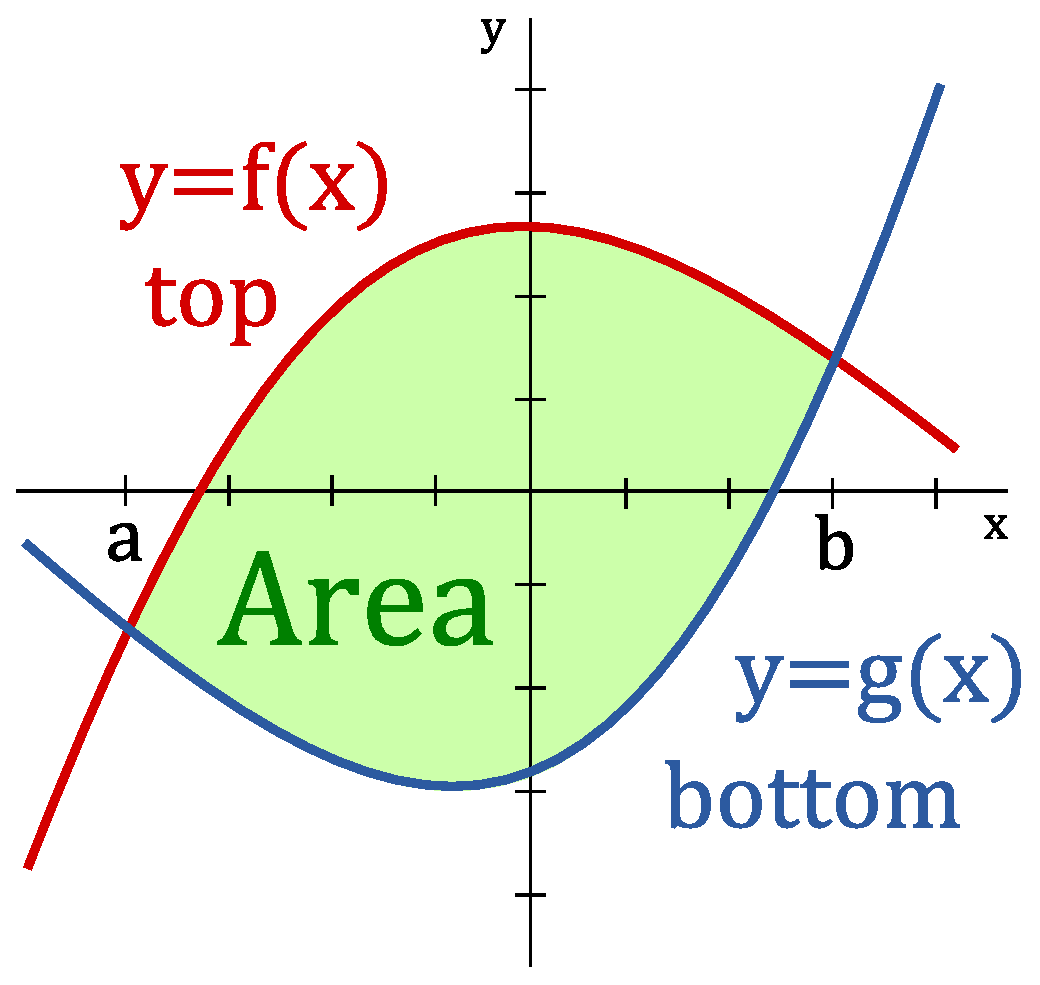
\includegraphics[width=2.5in]{images2/area-between-formula}$$
%
%More formally, the area $A$ of the region bounded by the curves $y=f(x)$ and $y=g(x)$ and the lines $x=a$ and $x=b$ is:
%$$A=\int_a^b\left|f(x)-g(x)\right|\,dx.$$
%
%\begin{example}{Area between Curves} {AreaBetweenCurves4} 
%Find the area between $\ds f(x)= -x^2+4x$ and
%$\ds g(x)=x^2-6x+5$; the
% curves are shown in figure~\xrefn{fig:area bounded by curves}. 
%\end{example}
%
%\begin{solution} 
%Here we
%are not given a specific interval, so it must be the case that there
%is a ``natural'' region involved. Since the curves are both parabolas,
%the only reasonable interpretation is the region between the two
%intersection points, which can be computed as:
%$${5\pm\sqrt{15}\over2}.$$
%If we let $\ds a=(5-\sqrt{15})/2$ and $\ds b=(5+\sqrt{15})/2$,
%the total area is 
%\begin{eqnarray*}
%  \int_a^b -x^2+4x-(x^2-6x+5)\,dx
%  &=&\int_a^b -2x^2+10x-5\,dx\cr
%  &=&\left.-{2x^3\over3}+5x^2-5x\right|_a^b\cr
%  &=&5\sqrt{15}.\cr
%\end{eqnarray*}
%after a bit of simplification.
%\end{solution}
%
%\figure[H]
%\centerline{\vbox{\beginpicture
%\normalgraphs
%%\ninepoint
%\setcoordinatesystem units <1.7truecm,0.4truecm>
%\setplotarea x from 0 to 5, y from -5 to 5
%\axis left ticks numbered from -5 to 5 by 5 /
%\axis bottom shiftedto y=0 ticks numbered from 1 to 5 by 1 /
%\setquadratic
%\plot
%0.000 0.000 0.250 0.938 0.500 1.750 0.750 2.438 1.000 3.000 
%1.250 3.438 1.500 3.750 1.750 3.938 2.000 4.000 2.250 3.938 
%2.500 3.750 2.750 3.438 3.000 3.000 3.250 2.438 3.500 1.750 
%3.750 0.938 4.000 0.000 4.250 -1.062 4.500 -2.250 4.750 -3.562 
%5.000 -5.000 /
%\plot
%0.000 5.000 0.250 3.562 0.500 2.250 0.750 1.062 1.000 0.000 
%1.250 -0.938 1.500 -1.750 1.750 -2.438 2.000 -3.000 2.250 -3.438 
%2.500 -3.750 2.750 -3.938 3.000 -4.000 3.250 -3.938 3.500 -3.750 
%3.750 -3.438 4.000 -3.000 4.250 -2.438 4.500 -1.750 4.750 -0.938 
%5.000 0.000 /
%\endpicture}}
%\caption{Area bounded by two curves. \label{fig:area bounded by curves}}
%\endfigure
%
%Some general guidelines to compute the area between two curves follows.
%
%\begin{formulabox}[Guidelines for Area Between Two Curves]
%\begin{enumerate}
%	\item Find the intersection points.  
%	\item Draw a sketch of the two curves.  
%	\item Using the sketch determine which curve is the top curve and which curve is the bottom curve. You may need to split the area up into multiple regions if the curves intersect multiple times in $[a,b]$.
%	\item Put the above information into the appropriate formula (once for each region): 
%		$$\ffont{Area}=\int_a^b (\mbox{top curve}) - (\mbox{bottom curve})\,dx,\qquad a\leq x\leq b.$$
%	\item Evaluate the integral using the Fundamental Theorem of Calculus (you should get a positive number representing an area).
%\end{enumerate}
%\end{formulabox}
%



%%%%%%%%%%%%%%%%%%%%%%%%%%%%%%%%%%%%%%%%%%%%%%%%%

\Opensolutionfile{solutions}[ex]
\section*{Exercises for Section \ref{sec:AreaBetweenCurves}}

\begin{multicols}{2}[]

\begin{enumialphparenastyle}

% % % % % % % % % % % % % %

\begin{ex}
Find the area of the shaded region in the given graph.

\begin{enumerate}

\item {\begin{minipage}{\textwidth} 
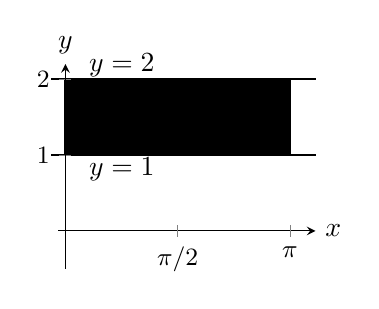
\begin{tikzpicture}
\begin{axis}[width=0.4\textwidth,%
tick label style={font=\small},axis y line=middle,axis x line=middle,name=myplot,axis on top,%
			%x=.37\marginparwidth,
			%y=.37\marginparwidth,
			xtick=\empty,% 
			extra x ticks={3.14,1.57},
			extra x tick labels={$\pi$,$\pi/2$},
			ytick={-1,1,2,3},
			%minor y tick num=1,%extra y ticks={-5,-3,...,7},%
%			minor x tick num=4,
			ymin=-.5,ymax=2.2,%
			xmin=-.1,xmax=3.5,%
			clip=false]

\addplot [{\coloronefill},stack plots=y,samples=40,domain=0:3.14] {1};
\addplot [{\coloronefill},thick,fill={\coloronefill},area style,stack plots=y,samples=40,domain=0:3.14] {1} \closedcycle;

\addplot [smooth,thick, {\colorone},samples=40, domain=-0.2:3.5] {1} node [shift={(-70pt,-5pt)} ,black] { $y=1$};

\addplot [smooth,thick, {\colorone},samples=40, domain=-0.2:3.5] {2} node [shift={(-70pt,5pt)} ,black] {  $y=2$};


\end{axis}

\node [right] at (myplot.right of origin) { $x$};
\node [above] at (myplot.above origin) {  $y$};
\end{tikzpicture}
\end{minipage}
}


\item {\begin{minipage}{\textwidth} 
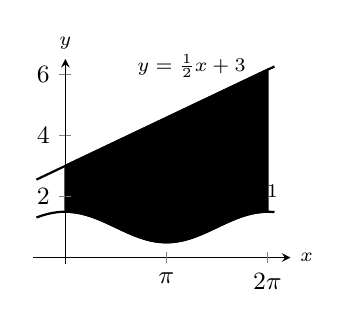
\begin{tikzpicture}
\begin{axis}[width=0.4\textwidth,%
tick label style={font=\small},axis y line=middle,axis x line=middle,name=myplot,axis on top,%
			%x=.37\marginparwidth,
			%y=.37\marginparwidth,
			xtick=\empty,% 
			extra x ticks={3.14,6.28},
			extra x tick labels={$\pi$,$2\pi$},
%			ytick=\empty,
			%minor y tick num=1,%extra y ticks={-5,-3,...,7},%
%			minor x tick num=4,
			ymin=-.2,ymax=6.5,%
			clip=false, % 
			xmin=-1,xmax=7%
]
\addplot [{\coloronefill},domain=0:6.28,stack plots=y,samples=40] {.5*cos(deg(x))+1};
\addplot [{\coloronefill},thick,fill={\coloronefill},area style,domain=0:6.28,stack plots=y,samples=40] {.5*x+3-(.5*cos(deg(x))+1)} \closedcycle;
\addplot [smooth,thick, {\colorone},domain=-.9:6.5,samples=40] {.5*cos(deg(x))+1} node [shift={(-25pt,7pt)} ,black] {\scriptsize $y=\frac12\cos x+1$};
\addplot [smooth,thick, {\colorone},domain=-.9:6.5,samples=40] {.5*x+3}node [shift={(-30pt,0pt)} ,black] {\scriptsize $y=\frac12x+3$};
\end{axis}

\node [right] at (myplot.right of origin) {\scriptsize $x$};
\node [above] at (myplot.above origin) {\scriptsize $y$};
\end{tikzpicture}
\end{minipage}}

\item {\begin{minipage}{\textwidth}
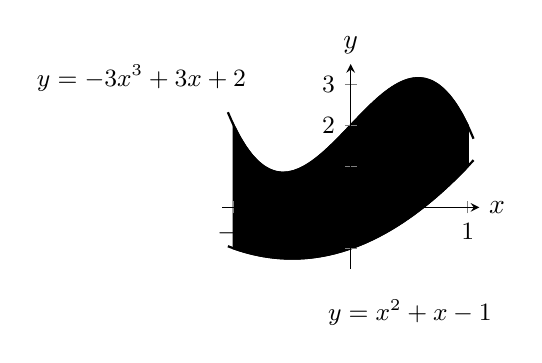
\begin{tikzpicture}
\begin{axis}[width=0.4\textwidth,%
tick label style={font=\small},axis y line=middle,axis x line=middle,name=myplot,axis on top,%
			%x=.37\marginparwidth,
			%y=.37\marginparwidth,
			xtick={-1,1},% 
%			extra x ticks={3.14,6.28},
%			extra x tick labels={$\pi$,$2\pi$},
			ytick={-1,1,2,3},
			%minor y tick num=1,%extra y ticks={-5,-3,...,7},%
%			minor x tick num=4,
			ymin=-1.5,ymax=3.5,%
			xmin=-1.1,xmax=1.1,%
			clip=false
]

\addplot [{\coloronefill},domain=-1:1,stack plots=y,samples=40] {x^2+x-1};
\addplot [{\coloronefill},thick,fill={\coloronefill},area style,domain=-1:1,stack plots=y,samples=40] {-3*x^3+3*x+2-(x^2+x-1)} \closedcycle;

\addplot [smooth,thick, {\colorone},domain=-1.05:1.05,samples=40] {x^2+x-1} node [shift={(-23pt,-55pt)} ,black] {\small $y=x^2+x-1$};

\addplot [smooth,thick, {\colorone},domain=-1.05:1.05,samples=40] {-3*x^3+3*x+2}node [shift={(-120pt,22pt)} ,black] {\small $y=-3x^3+3x+2$};


\end{axis}

\node [right] at (myplot.right of origin) {  $x$};
\node [above] at (myplot.above origin) {  $y$};
\end{tikzpicture}
\end{minipage}%\ifthenelse{\boolean{printquestions}}{\columnbreak}{}
}

\item {\begin{minipage}{\textwidth}
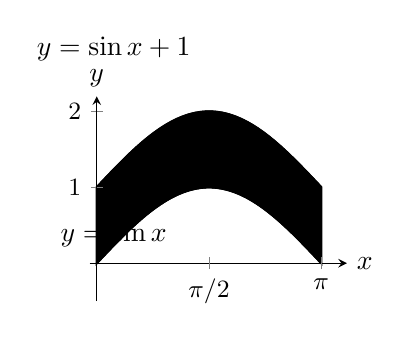
\begin{tikzpicture}
\begin{axis}[width=0.4\textwidth,%
tick label style={font=\small},axis y line=middle,axis x line=middle,name=myplot,axis on top,%
			%x=.37\marginparwidth,
			%y=.37\marginparwidth,
			xtick=\empty,% 
			extra x ticks={3.14,1.57},
			extra x tick labels={$\pi$,$\pi/2$},
			ytick={-1,1,2,3},
			%minor y tick num=1,%extra y ticks={-5,-3,...,7},%
%			minor x tick num=4,
			ymin=-.5,ymax=2.2,%
			xmin=-.1,xmax=3.5,%
			clip=false
]

\addplot [{\coloronefill},stack plots=y,samples=40,domain=0:3.14] {sin(deg(x))};
\addplot [{\coloronefill},thick,fill={\coloronefill},area style,stack plots=y,samples=40,domain=0:3.14] {sin(deg(x))+1-(sin(deg(x)))} \closedcycle;

\addplot [smooth,thick, {\colorone},samples=40,domain=0:3.14] {sin(deg(x))} node [shift={(-75pt,10pt)} ,black] { $y=\sin x$};

\addplot [smooth,thick, {\colorone},samples=40,domain=0:3.14] {sin(deg(x))+1} node [shift={(-75pt,50pt)} ,black] { $y=\sin x+1$};


\end{axis}

\node [right] at (myplot.right of origin) { $x$};
\node [above] at (myplot.above origin) { $y$};
\end{tikzpicture}
\end{minipage}
}
\item {\begin{minipage}{\textwidth} 
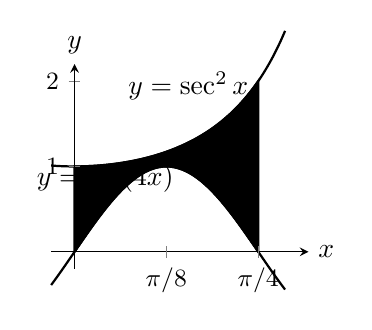
\begin{tikzpicture}
\begin{axis}[width=0.4\textwidth,%
tick label style={font=\small},axis y line=middle,axis x line=middle,name=myplot,axis on top,%
			%x=.37\marginparwidth,
			%y=.37\marginparwidth,
			xtick=\empty,% 
			extra x ticks={.785,.392},
			extra x tick labels={$\pi/4$,$\pi/8$},
			ytick={-1,1,2,3},
			%minor y tick num=1,%extra y ticks={-5,-3,...,7},%
%			minor x tick num=4,
			ymin=-.2,ymax=2.2,%
			xmin=-.1,xmax=1,%
			clip=false
]

\addplot [{\coloronefill},stack plots=y,samples=40,domain=0:.785] {sin(deg(4*x))};
\addplot [{\coloronefill},thick,fill={\coloronefill},area style,stack plots=y,samples=40,domain=0:.785] {sec(deg(x))^2-(sin(deg(4*x)))} \closedcycle;

\addplot [smooth,thick, {\colorone},domain=-.1:.9,samples=60] {sin(deg(4*x))} node [shift={(-65pt,40pt)} ,black] {  $y=\sin (4x)$};

\addplot [smooth,thick, {\colorone},domain=-.1:.9,samples=60] {sec(deg(x))^2} node [shift={(-35pt,-20pt)} ,black] {  $y=\sec^2 x$};
\end{axis}

\node [right] at (myplot.right of origin) {  $x$};
\node [above] at (myplot.above origin) {  $y$};
\end{tikzpicture}
\end{minipage}}

\item {\begin{minipage}{\textwidth}
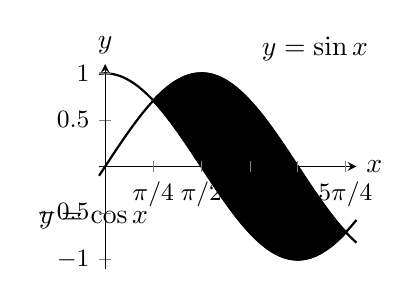
\begin{tikzpicture}
\begin{axis}[width=0.4\textwidth,%
tick label style={font=\small},axis y line=middle,axis x line=middle,name=myplot,axis on top,%
			%x=.37\marginparwidth,
			%y=.37\marginparwidth,
			xtick=\empty,% 
			extra x ticks={.785,1.57,2.36,3.14,3.92},
			extra x tick labels={$\pi/4$,$\pi/2$,$3\pi/4$,$\pi$,$5\pi/4$},
%			ytick={-1,1,2,3},
			%minor y tick num=1,%extra y ticks={-5,-3,...,7},%
%			minor x tick num=4,
			ymin=-1.1,ymax=1.1,%
			xmin=-.1,xmax=4.1,%
			clip=false
]

\addplot [{\coloronefill},stack plots=y,samples=40,domain=.785:3.92] {cos(deg(x))};
\addplot [{\coloronefill},thick,fill={\coloronefill},area style,stack plots=y,samples=40,domain=.785:3.92] {sin(deg(x))-(cos(deg(x)))} \closedcycle;

\addplot [smooth,thick, {\colorone},domain=-.1:4.1,samples=40] {sin(deg(x))} node [shift={(-15pt,70pt)} ,black] {  $y=\sin x$};

\addplot [smooth,thick, {\colorone},domain=-.1:4.1,samples=40] {cos(deg(x))} node [shift={(-95pt,0pt)} ,black] {  $y=\cos x$};


\end{axis}

\node [right] at (myplot.right of origin) {  $x$};
\node [above] at (myplot.above origin) {  $y$};
\end{tikzpicture}
\end{minipage}
}

\item {\begin{minipage}{\linewidth} 
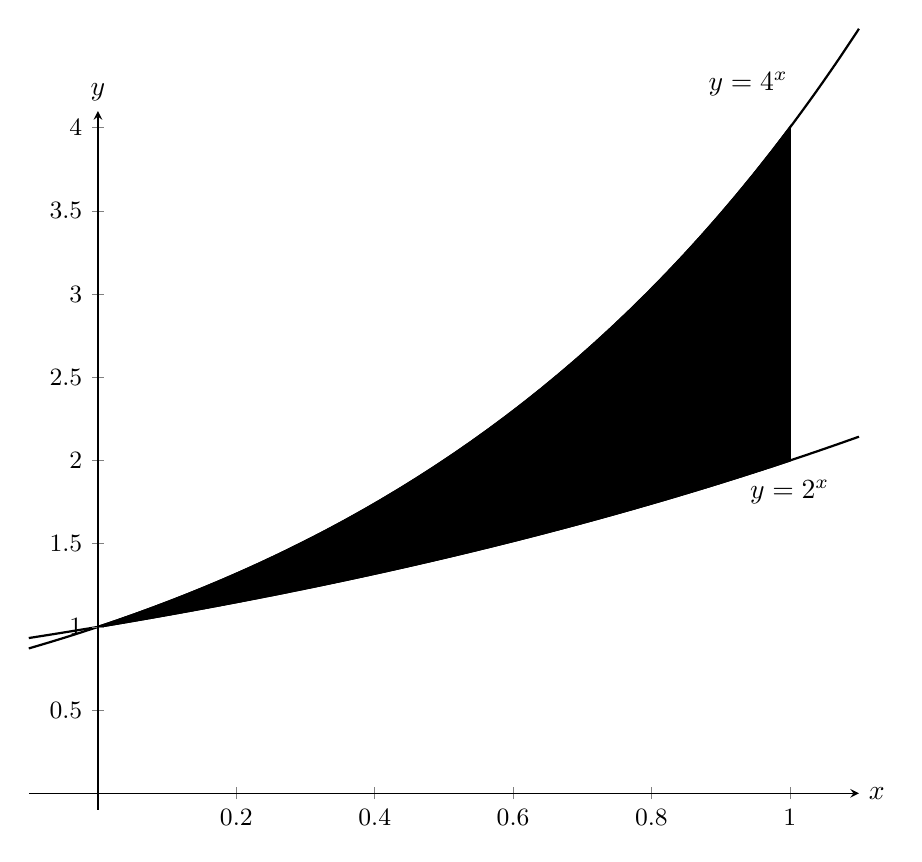
\begin{tikzpicture}
\begin{axis}[width=\linewidth,%
tick label style={font=\small},axis y line=middle,axis x line=middle,name=myplot,axis on top,%
			%x=.37\marginparwidth,
			%y=.37\marginparwidth,
%			xtick=\empty,% 
%			extra x ticks={.785,1.57,2.36,3.14,3.92},
%			extra x tick labels={$\pi/4$,$\pi/2$,$3\pi/4$,$\pi$,$5\pi/4$},
%			ytick={-1,1,2,3},
			%minor y tick num=1,%extra y ticks={-5,-3,...,7},%
%			minor x tick num=4,
			ymin=-.1,ymax=4.1,%
			xmin=-.1,xmax=1.1,%
						clip=false]

\addplot [{\coloronefill},stack plots=y,samples=40,domain=0:1] {2^x};
\addplot [{\coloronefill},thick,fill={\coloronefill},area style,stack plots=y,samples=40,domain=0:1] {4^x-(2^x)} \closedcycle;

\addplot [smooth,thick, {\colorone},domain=-.1:1.1,samples=40] {2^x} node [shift={(-25pt,-20pt)} ,black] {  $y=2^x$};

\addplot [smooth,thick, {\colorone},domain=-.1:1.1,samples=40] {4^x} node [shift={(-40pt,-20pt)} ,black] {  $y=4^x$};


\end{axis}

\node [right] at (myplot.right of origin) {  $x$};
\node [above] at (myplot.above origin) {  $y$};
\end{tikzpicture}

\end{minipage}}



\end{enumerate}

\begin{sol}
\begin{enumerate}
\item {$\pi$}
\item {$4\pi+\pi^2\approx 22.436$}  
\item {$16/3$}
\item {$\pi$}
\item {$1/2$}
\item {$2\sqrt{2}$}
\item {$1/\ln 4$}
\end{enumerate}
\end{sol}
\end{ex}
% % % % % % % % % % % % % % % % %


\begin{ex}
Find the area of the enclosed region in two ways:\\
(1)	by treating the boundaries as functions of $x$, and\\
(2) by treating the boundaries as functions of $y$.
\begin{enumerate}
\item {\begin{minipage}{\textwidth} 
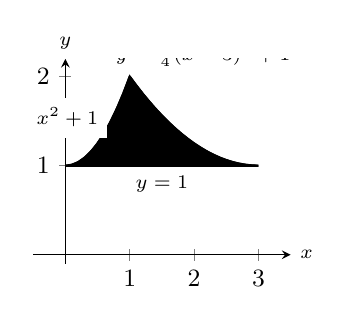
\begin{tikzpicture}
\begin{axis}[width=0.4\textwidth,%
tick label style={font=\small},axis y line=middle,axis x line=middle,name=myplot,%
			%x=.37\marginparwidth,
			%y=.37\marginparwidth,
%			xtick=\empty,% 
%			extra x ticks={3.14,1.57},
%			extra x tick labels={$\pi$,$\pi/2$},
%			ytick={-1,1,2,3},
			%minor y tick num=1,%extra y ticks={-5,-3,...,7},%
%			minor x tick num=4,
			ymin=-.1,ymax=2.2,%
			xmin=-.5,xmax=3.5%
]

%\addplot [{\coloronefill},stack plots=y,samples=40,domain=0:3.14] {1};
%\addplot [{\coloronefill},thick,fill={\coloronefill},area style,stack plots=y,samples=40,domain=0:3.14] {1} \closedcycle;

\addplot [thick, {\coloronefill},fill={\coloronefill}] coordinates { (0,1.)(0.1,1.01)(0.2,1.04)(0.3,1.09)(0.4,1.16)(0.5,1.25)(0.6,1.36)(0.7,1.49)(0.8,1.64)(0.9,1.81)(1.,2.)(1.1,1.903)(1.2,1.81)(1.3,1.723)(1.4,1.64)(1.5,1.563)(1.6,1.49)(1.7,1.423)(1.8,1.36)(1.9,1.303)(2.,1.25)(2.1,1.203)(2.2,1.16)(2.3,1.123)(2.4,1.09)(2.5,1.063)(2.6,1.04)(2.7,1.023)(2.8,1.01)(2.9,1.003)(3.,1.)(0,1)};

\addplot [smooth,thick, {\colorone},samples=40,domain=0:1] {x^2+1} node [shift={(-30pt,-15pt)} ,black,fill=white] {\scriptsize $y=x^2+1$};

\addplot [smooth,thick, {\colorone},samples=40,domain=1:3] {.25*(x-3)^2+1} node [shift={(-20pt,40pt)} ,black] {\scriptsize $y=\frac14(x-3)^2+1$};

\draw [smooth,thick, {\colorone}] (axis cs:0,1) --  node [pos=.5,below,black] {\scriptsize $y=1$} (axis cs:3,1);

\end{axis}

\node [right] at (myplot.right of origin) {\scriptsize $x$};
\node [above] at (myplot.above origin) {\scriptsize $y$};
\end{tikzpicture}
\end{minipage}}

\item {\begin{minipage}{\textwidth} 
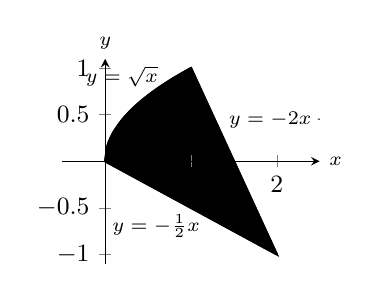
\begin{tikzpicture}
\begin{axis}[width=0.4\textwidth,%
tick label style={font=\small},axis y line=middle,axis x line=middle,name=myplot,axis on top,%
			%x=.37\marginparwidth,
			%y=.37\marginparwidth,
%			xtick=\empty,% 
%			extra x ticks={3.14,1.57},
%			extra x tick labels={$\pi$,$\pi/2$},
%			ytick={-1,1,2,3},
			%minor y tick num=1,%extra y ticks={-5,-3,...,7},%
%			minor x tick num=4,
			ymin=-1.1,ymax=1.1,%
			xmin=-.5,xmax=2.5%
]

\addplot [thick, {\coloronefill},fill={\coloronefill}] coordinates { (0,0)(0.02,0.1414)(0.04,0.2)(0.06,0.2449)(0.08,0.2828)(0.1,0.3162)(0.2,0.4472)(0.3,0.5477)(0.4,0.6325)(0.5,0.7071)(0.6,0.7746)(0.7,0.8367)(0.8,0.8944)(0.9,0.9487)(1.,1.)(2,-1)(0,0)};

\addplot [smooth,thick, {\colorone},samples=40,domain=0:1] {sqrt(x)} node [shift={(-25pt,-3pt)} ,black] {\scriptsize $y=\sqrt{x}$};
%
%\addplot [smooth,thick, {\colorone},samples=40,domain=1:3] {.25*(x-3)^2+1} node [shift={(-25pt,25pt)} ,black] {\scriptsize $y=x^2+1$};
%
\draw [smooth,thick, {\colorone}] (axis cs:1,1) --  node [pos=.5,shift={(20pt,15pt)},black] {\scriptsize $y=-2x+3$} (axis cs:2,-1);

\draw [smooth,thick, {\colorone}] (axis cs:2,-1) --  node [pos=.3,shift={(-25pt,0pt)},black] {\scriptsize $y=-\frac12x$} (axis cs:0,0);

\end{axis}

\node [right] at (myplot.right of origin) {\scriptsize $x$};
\node [above] at (myplot.above origin) {\scriptsize $y$};
\end{tikzpicture}
\end{minipage}}

\item {\begin{minipage}{\textwidth} 
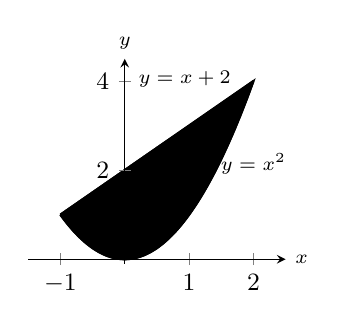
\begin{tikzpicture}
\begin{axis}[width=0.4\textwidth,%
tick label style={font=\small},axis y line=middle,axis x line=middle,name=myplot,axis on top,%
			%x=.37\marginparwidth,
			%y=.37\marginparwidth,
%			xtick=\empty,% 
%			extra x ticks={3.14,1.57},
%			extra x tick labels={$\pi$,$\pi/2$},
%			ytick={-1,1,2,3},
			%minor y tick num=1,%extra y ticks={-5,-3,...,7},%
%			minor x tick num=4,
			ymin=-.1,ymax=4.5,%
			xmin=-1.5,xmax=2.5%
]

\addplot [thick, {\coloronefill},fill={\coloronefill}] coordinates { (-1.,1.)(-0.9,0.81)(-0.8,0.64)(-0.7,0.49)(-0.6,0.36)(-0.5,0.25)(-0.4,0.16)(-0.3,0.09)(-0.2,0.04)(-0.1,0.01)(0,0)(0.1,0.01)(0.2,0.04)(0.3,0.09)(0.4,0.16)(0.5,0.25)(0.6,0.36)(0.7,0.49)(0.8,0.64)(0.9,0.81)(1.,1.)(1.1,1.21)(1.2,1.44)(1.3,1.69)(1.4,1.96)(1.5,2.25)(1.6,2.56)(1.7,2.89)(1.8,3.24)(1.9,3.61)(2.,4.)(-1,1)};

\addplot [smooth,thick, {\colorone},samples=40,domain=-1:2] {x^2} node [shift={(0pt,-30pt)} ,black] {\scriptsize $y=x^2$};
%
%\addplot [smooth,thick, {\colorone},samples=40,domain=1:3] {.25*(x-3)^2+1} node [shift={(-25pt,25pt)} ,black] {\scriptsize $y=x^2+1$};
%
\draw [smooth,thick, {\colorone}] (axis cs:2,4) --  node [pos=.5,shift={(10pt,25pt)},black] {\scriptsize $y=x+2$} (axis cs:-1,1);

%\draw [smooth,thick, {\colorone}] (axis cs:2,-1) --  node [pos=.3,shift={(-25pt,0pt)},black] {\scriptsize $y=-1/2x$} (axis cs:0,0);

\end{axis}

\node [right] at (myplot.right of origin) {\scriptsize $x$};
\node [above] at (myplot.above origin) {\scriptsize $y$};
\end{tikzpicture}
\end{minipage}}


\item {\begin{minipage}{\textwidth} 
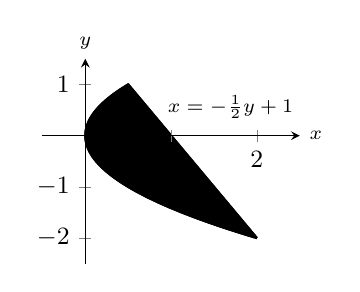
\begin{tikzpicture}
\begin{axis}[width=0.4\textwidth,%
tick label style={font=\small},axis y line=middle,axis x line=middle,name=myplot,axis on top,%
			%x=.37\marginparwidth,
			%y=.37\marginparwidth,
%			xtick=\empty,% 
%			extra x ticks={3.14,1.57},
%			extra x tick labels={$\pi$,$\pi/2$},
%			ytick={-1,1,2,3},
			%minor y tick num=1,%extra y ticks={-5,-3,...,7},%
%			minor x tick num=4,
			ymin=-2.5,ymax=1.5,%
			xmin=-.5,xmax=2.5%
]

\addplot [thick, {\coloronefill},fill={\coloronefill}] coordinates { (2.,-2.)(1.805,-1.9)(1.62,-1.8)(1.445,-1.7)(1.28,-1.6)(1.125,-1.5)(0.98,-1.4)(0.845,-1.3)(0.72,-1.2)(0.605,-1.1)(0.5,-1.)(0.405,-0.9)(0.32,-0.8)(0.245,-0.7)(0.18,-0.6)(0.125,-0.5)(0.08,-0.4)(0.045,-0.3)(0.02,-0.2)(0.005,-0.1)(0,0)(0.005,0.1)(0.02,0.2)(0.045,0.3)(0.08,0.4)(0.125,0.5)(0.18,0.6)(0.245,0.7)(0.32,0.8)(0.405,0.9)(0.5,1.)(2,-2)};

\addplot [smooth,thick, {\colorone},samples=40,domain=-2:1] ({.5*x^2},x) node [shift={(5pt,-70pt)} ,black] {\scriptsize $x=\frac12y^2$};
%
%\addplot [smooth,thick, {\colorone},samples=40,domain=1:3] {.25*(x-3)^2+1} node [shift={(-25pt,25pt)} ,black] {\scriptsize $y=x^2+1$};
%
\draw [smooth,thick, {\colorone}] (axis cs:2,-2) --  node [pos=.85,shift={(30pt,0pt)},black] {\scriptsize $x=-\frac12y+1$} (axis cs:.5,1);

%\draw [smooth,thick, {\colorone}] (axis cs:2,-1) --  node [pos=.3,shift={(-25pt,0pt)},black] {\scriptsize $y=-1/2x$} (axis cs:0,0);

\end{axis}

\node [right] at (myplot.right of origin) {\scriptsize $x$};
\node [above] at (myplot.above origin) {\scriptsize $y$};
\end{tikzpicture}
\end{minipage}}



\item {\begin{minipage}{\textwidth} 
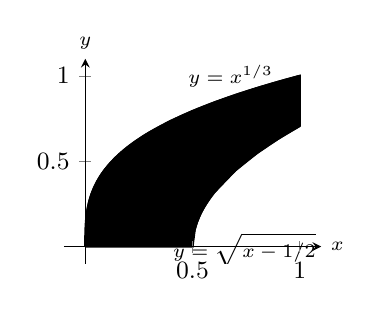
\begin{tikzpicture}
\begin{axis}[width=0.4\textwidth,%
tick label style={font=\small},axis y line=middle,axis x line=middle,name=myplot,axis on top,%
			%x=.37\marginparwidth,
			%y=.37\marginparwidth,
%			xtick=\empty,% 
%			extra x ticks={3.14,1.57},
%			extra x tick labels={$\pi$,$\pi/2$},
%			ytick={-1,1,2,3},
			%minor y tick num=1,%extra y ticks={-5,-3,...,7},%
%			minor x tick num=4,
			ymin=-.1,ymax=1.1,%
			xmin=-.1,xmax=1.1%
]

\addplot [thick, {\coloronefill},fill={\coloronefill}] coordinates { (0,0)(0.01,0.2154)(0.02,0.2714)(0.03,0.3107)(0.04,0.342)(0.05,0.3684)(0.06,0.3915)(0.07,0.4121)(0.08,0.4309)(0.09,0.4481)(0.1,0.4642)(0.12,0.4932)(0.14,0.5192)(0.16,0.5429)(0.18,0.5646)(0.2,0.5848)(0.22,0.6037)(0.24,0.6214)(0.26,0.6383)(0.28,0.6542)(0.3,0.6694)(0.4,0.7368)(0.5,0.7937)(0.6,0.8434)(0.7,0.8879)(0.8,0.9283)(0.9,0.9655)(1.,1.)(1.,0.7071)(0.9,0.6325)(0.8,0.5477)(0.7,0.4472)(0.6,0.3162)(0.59,0.3)(0.58,0.2828)(0.57,0.2646)(0.56,0.2449)(0.55,0.2236)(0.54,0.2)(0.53,0.1732)(0.52,0.1414)(0.51,0.1)(0.5,0)(0,0)};

\addplot [smooth,thick, {\colorone},samples=40,domain=0:1] (x^3,x) node [shift={(-25pt,0pt)} ,black] {\scriptsize $y=x^{1/3}$};
%
\addplot [smooth,thick, {\colorone},samples=40,domain=0:.7071] ({(x)^2+.5},x) node [shift={(-20pt,-45pt)} ,black] {\scriptsize $y=\sqrt{x-1/2}$};
%
%\draw [smooth,thick, {\colorone}] (axis cs:2,-2) --  node [pos=.85,shift={(30pt,0pt)},black] {\scriptsize $x=-1/2y+1$} (axis cs:.5,1);

%\draw [smooth,thick, {\colorone}] (axis cs:2,-1) --  node [pos=.3,shift={(-25pt,0pt)},black] {\scriptsize $y=-1/2x$} (axis cs:0,0);

\end{axis}

\node [right] at (myplot.right of origin) {\scriptsize $x$};
\node [above] at (myplot.above origin) {\scriptsize $y$};
\end{tikzpicture}
\end{minipage}}
\end{enumerate}		

\begin{sol}
\begin{enumerate}
\item {$1$}
\item {$5/3$}
\item {$9/2$}
\item {$9/4$}
\item {$1/12(9-2\sqrt{2})\approx 0.514$}
\end{enumerate}		
\end{sol}


\end{ex}


\begin{ex}
\begin{enumerate}
\item {$(1,1)$,\quad $(2,3)$,\quad and \quad $(3,3)$}
\item {$(-1,1)$,\quad $(1,3)$,\quad and \quad $(2,-1)$}
\item {$(1,1)$,\quad $(3,3)$,\quad and \quad $(3,3)$}
\item {$(0,0)$,\quad $(2,5)$,\quad and \quad $(5,2)$}
\end{enumerate}

\begin{sol}
\begin{enumerate}
\item $ 1 $
\item $ 5 $
\item $ 4 $
\item $ \frac{133}{20} $
\end{enumerate}
\end{sol}

\end{ex}


Find the area bounded by the curves.

%%%%%%%%%%
\begin{ex}
 $\ds y=x^4-x^2$ and $\ds y=x^2$ (the part to the right of the $y$-axis)
\begin{sol}
 $\ds 8\sqrt2/15$
\end{sol}
\end{ex}

%%%%%%%%%%
\begin{ex}
 $\ds x=y^3$ and $\ds x=y^2$
\begin{sol}
 $1/12$
\end{sol}
\end{ex}

%%%%%%%%%%
\begin{ex}
 $\ds x=1-y^2$ and $y=-x-1$
\begin{sol}
 $9/2$
\end{sol}
\end{ex}

%%%%%%%%%%
\begin{ex}
 $\ds x=3y-y^2$ and $x+y=3$
\begin{sol}
 $4/3$
\end{sol}
\end{ex}

%%%%%%%%%%
\begin{ex}
 $y=\cos(\pi x/2)$ and $\ds y=1- x^2$ (in the first quadrant)
\begin{sol}
 $2/3-2/\pi$
\end{sol}
\end{ex}

%%%%%%%%%%
\begin{ex}
 $y=\sin(\pi x/3)$ and $y=x$ (in the first quadrant)
\begin{sol}
 $\ds 3/\pi - 3\sqrt3/(2\pi)-1/8$
\end{sol}
\end{ex}

%%%%%%%%%%
\begin{ex}
 $\ds y=\sqrt{x}$ and $\ds y=x^2$
\begin{sol}
 $1/3$
\end{sol}
\end{ex}

%%%%%%%%%%
\begin{ex}
 $\ds y=\sqrt x$ and $\ds y=\sqrt{x+1}$, $0\le x\le 4$
\begin{sol}
 $\ds 10\sqrt{5}/3-6$
\end{sol}
\end{ex}

%%%%%%%%%%
\begin{ex}
 $x=0$ and $\ds x=25-y^2$
\begin{sol}
 $500/3$
\end{sol}
\end{ex}

%%%%%%%%%%
\begin{ex}
 $y=\sin x\cos x$ and $y=\sin x$, $0\le x\le \pi$
\begin{sol}
 $2$
\end{sol}
\end{ex}

%%%%%%%%%%
\begin{ex}
 $\ds y=x^{3/2}$ and $\ds y=x^{2/3}$
\begin{sol}
 $1/5$
\end{sol}
\end{ex}

%%%%%%%%%%
\begin{ex}
 $\ds y=x^2-2x$ and $y=x-2$
\begin{sol}
 $1/6$
\end{sol}
\end{ex}

%%%%%%%%%%
\begin{ex}
{Use the Trapezoidal Rule to approximate the area of the pictured lake whose lengths, in hundreds of meters, are measured in $ 100 $-m. increments.\label{07_01_ex_29}

\begin{center}

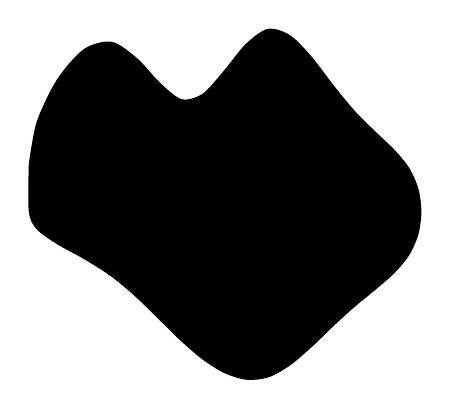
\begin{tikzpicture}[yscale=.6]%[width=\marginparwidth+25pt]
%\begin{axis}[width=\marginparwidth+25pt,%
%tick label style={font=\scriptsize},axis y line=middle,axis x line=middle,name=myplot,axis on top,%
%			%x=.37\marginparwidth,
%			%y=.37\marginparwidth,
%			xtick={1,2,3,4,5,6,7,8,9,10,11,12},% 
%%			extra x ticks={12.57},
%%			extra x tick labels={$4\pi$},
%%			ytick=\empty,
%			%minor y tick num=1,%extra y ticks={-5,-3,...,7},%
%%			minor x tick num=4,
%			ymin=-.1,ymax=8.5,%
%			xmin=-.1,xmax=12.5%
%]

\draw [{\colorone},thick,fill={\coloronefill},smooth] plot coordinates {(0,1.)(0.1013,1.899)(0.3567,2.785)(0.6934,3.42)(1.039,3.569)(1.355,3.224)(1.646,2.705)(1.925,2.355)(2.2,2.473)(2.475,2.968)(2.75,3.529)(3.025,3.844)(3.3,3.709)(3.575,3.249)(3.85,2.651)(4.125,2.098)(4.389,1.661)(4.624,1.285)(4.807,0.9071)(4.921,0.4743)(4.958,0)(4.921,-0.4743)(4.807,-0.9071)(4.624,-1.279)(4.389,-1.625)(4.125,-1.986)(3.85,-2.401)(3.575,-2.843)(3.3,-3.233)(3.025,-3.487)(2.75,-3.536)(2.475,-3.397)(2.2,-3.111)(1.925,-2.718)(1.646,-2.263)(1.355,-1.792)(1.039,-1.352)(0.6934,-0.9844)(0.3567,-0.6744)(0.1013,-0.3653)(0,0)(0,1)};

\draw (1,3.56) -- (1,-1.35) node [shift={(-3pt,0pt)},rotate=90,pos=.5] {\scriptsize 4.9};

\draw (2,2.37) -- (2,-2.8) node [shift={(-3pt,0pt)},rotate=90,pos=.5] {\scriptsize 5.2};

\draw (3,3.8) -- (3,-3.5) node [shift={(-3pt,0pt)},rotate=90,pos=.5] {\scriptsize 7.3};

\draw (4,2.35) -- (4,-2.15) node [shift={(-3pt,0pt)},rotate=90,pos=.5] {\scriptsize 4.5};

%\end{axis}
%
%\node [right] at (myplot.right of origin) {\scriptsize $x$};
%\node [above] at (myplot.above origin) {\scriptsize $y$};
\end{tikzpicture}
\end{center}}


\begin{sol}
{219,000 m$^2$}
\end{sol}
\end{ex}

%%%%%%%%%%
\begin{ex}
{Use Simpson's Rule to approximate the area of the pictured lake whose lengths, in hundreds of meters, are measured in 200-meter increments.\label{07_01_ex_30}

\begin{center}
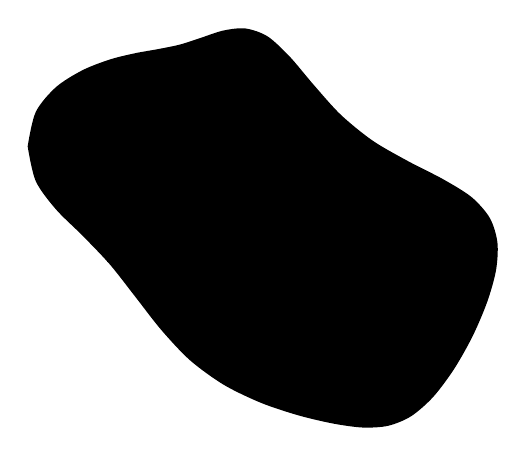
\begin{tikzpicture}[yscale=.6]%[width=\marginparwidth+25pt]
%\begin{axis}[width=\marginparwidth+25pt,%
%tick label style={font=\scriptsize},axis y line=middle,axis x line=middle,name=myplot,axis on top,%
%			%x=.37\marginparwidth,
%			%y=.37\marginparwidth,
%			xtick={1,2,3,4,5,6,7,8,9,10,11,12},% 
%%			extra x ticks={12.57},
%%			extra x tick labels={$4\pi$},
%%			ytick=\empty,
%			%minor y tick num=1,%extra y ticks={-5,-3,...,7},%
%%			minor x tick num=4,
%			ymin=-.1,ymax=8.5,%
%			xmin=-.1,xmax=12.5%
%]

\draw [{\colorone},thick,fill={\coloronefill},smooth] plot coordinates {(0,2.)(0.1013,2.717)(0.3567,3.238)(0.6934,3.594)(1.039,3.818)(1.355,3.948)(1.646,4.035)(1.925,4.132)(2.2,4.28)(2.475,4.428)(2.75,4.471)(3.025,4.307)(3.305,3.88)(3.607,3.287)(3.952,2.652)(4.361,2.098)(4.815,1.661)(5.253,1.285)(5.614,0.9071)(5.843,0.4705)(5.938,-0.04167)(5.919,-0.6295)(5.807,-1.293)(5.624,-2.009)(5.389,-2.703)(5.125,-3.29)(4.849,-3.692)(4.562,-3.892)(4.243,-3.929)(3.871,-3.846)(3.432,-3.674)(2.956,-3.409)(2.484,-3.028)(2.057,-2.511)(1.692,-1.869)(1.363,-1.168)(1.039,-0.4819)(0.6934,0.1248)(0.3567,0.679)(0.1013,1.273)(0,2.)};

\draw (1,3.8) -- (1,-.45) node [shift={(-3pt,0pt)},rotate=90,pos=.5] {\scriptsize 4.25};
%
\draw (2,4.15) -- (2,-2.45) node [shift={(-3pt,0pt)},rotate=90,pos=.5] {\scriptsize 6.6};

\draw (3,4.3) -- (3,-3.4) node [shift={(-3pt,0pt)},rotate=90,pos=.5] {\scriptsize 7.7};

\draw (4,2.6) -- (4,-3.85) node [shift={(-3pt,0pt)},rotate=90,pos=.5] {\scriptsize 6.45};

\draw (5,1.45) -- (5,-3.45) node [shift={(-3pt,0pt)},rotate=90,pos=.5] {\scriptsize 4.9};

%\end{axis}
%
%\node [right] at (myplot.right of origin) {\scriptsize $x$};
%\node [above] at (myplot.above origin) {\scriptsize $y$};
\end{tikzpicture}



\end{center}}

\begin{sol}
{623,333 m$^2$}

\end{sol}
\end{ex}


\end{enumialphparenastyle}

\end{multicols}
\clearpage 